\documentclass{beamer}
\usetheme[
  sectionpage=progressbar,
  numbering=counter,
  titleformat=smallcaps
  % progressbar=frametitle
]{metropolis}             % Use metropolis theme

% Fix needed to make fonts work on ubuntu: https://github.com/matze/mtheme/issues/280
%\setsansfont[	 	  
%    Extension      = .otf,
%    UprightFont    = *-Light,
%    ItalicFont     = *-LightItalic,
%    BoldFont       = *-Regular,
%    BoldItalicFont = *-RegularItalic
%]{FiraSans}
%\setmonofont[
%    Extension   = .otf,
%    UprightFont = *-Regular,
%    BoldFont    = *-Medium
%]{FiraMono}

\usepackage[german]{babel}
\usepackage{xcolor}
\usepackage{hyperref}

\newcommand\ytl[2]{
  \parbox[b]{8em}{\hfill{\color{cyan}\bfseries\sffamily #1}~$\cdots\cdots$~}\makebox[0pt][c]{$\bullet$}\vrule\quad \parbox[c]{4.5cm}{\vspace{7pt}\color{red!40!black!80}\raggedright\sffamily #2.\\[7pt]}\\[-3pt]
}


\definecolor{cioDarkBlue}{HTML}{12254c}
\setbeamercolor{normal text}{%
    fg=cioDarkBlue,
    bg=black!2
}

\graphicspath{{img/}}

\title{Eigenes VPN mit Wireguard}
\date{28.9.2019}
\author{Anian Ziegler}
\institute{Hackerkiste 2019}

\begin{document}
  \maketitle

  % % % % % % % % % % % % % % % % % % % % % % %
  % Was ist das und für was braucht man das?  %
  % % % % % % % % % % % % % % % % % % % % % % % 
  \section{VPN? Was ist das und warum braucht man das?}

  \begin{frame}{Woher man VPNs kennt}
    \begin{center}
      Uni VPN oder Firmen VPNs \\
      \vspace{10pt}
      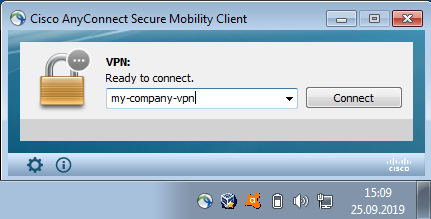
\includegraphics[width=\textwidth]{any-connect}
    \end{center}
  \end{frame}
  \begin{frame}{Woher man VPNs kennt}
    \begin{center}
      Komerzielle VPNs für Privatsphäre oder um Geoblocking zu umgehen \\
      \vspace{10pt}
      
\includegraphics[width=0.45\textwidth]{expressvpn}
      
\includegraphics[width=0.45\textwidth]{private-internet-access}
    \end{center}
  \end{frame}

  % - Nicht alle Tunnel sind VPNs aber alle VPNs sind Tunnel
  % - Man macht IP über IP 
  {
    \usebackgroundtemplate{
\includegraphics[width=\paperwidth]{tunnel-empty}}
    \begin{frame}{Tunnel}
    \end{frame}
  }
  {
    \usebackgroundtemplate{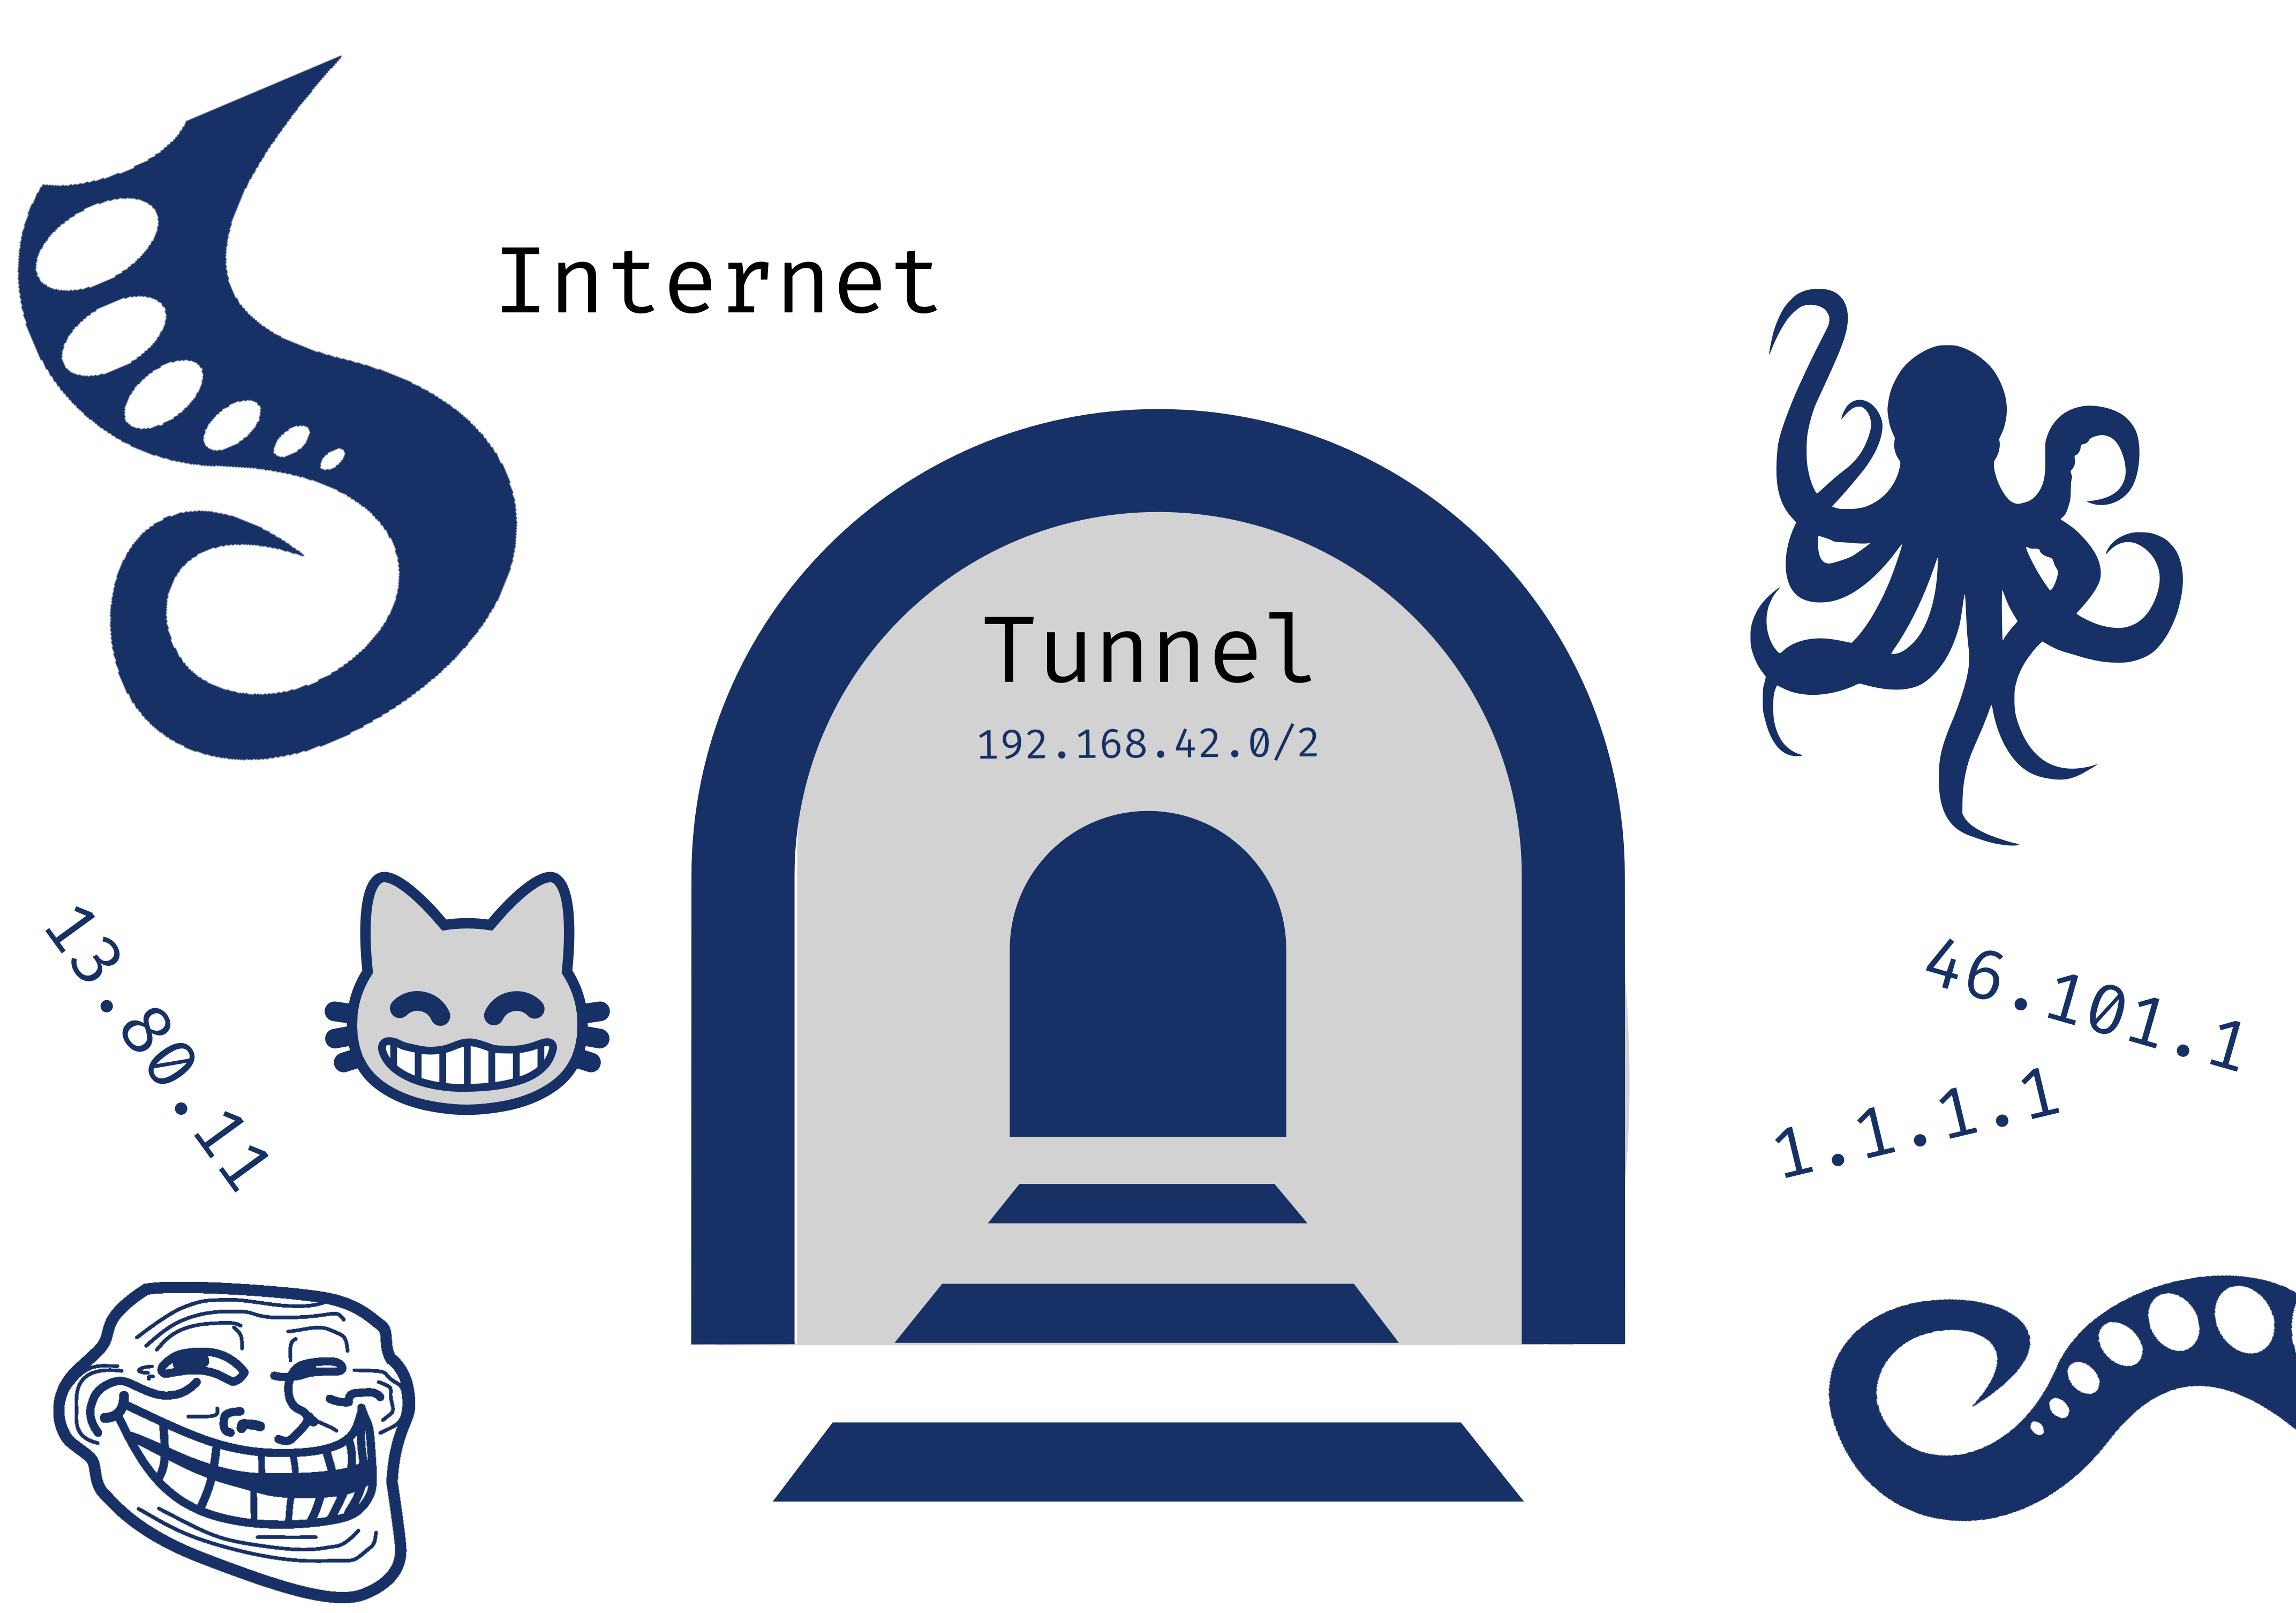
\includegraphics[width=\paperwidth]{tunnel-full}}
    \begin{frame}{Virtual Private Network}
    \end{frame}
  }
  {
    \usebackgroundtemplate{
\includegraphics[width=\paperwidth]{network-blue}}
    \begin{frame}{Virtual Private Network}
    \end{frame}
  }
  {
    \usebackgroundtemplate{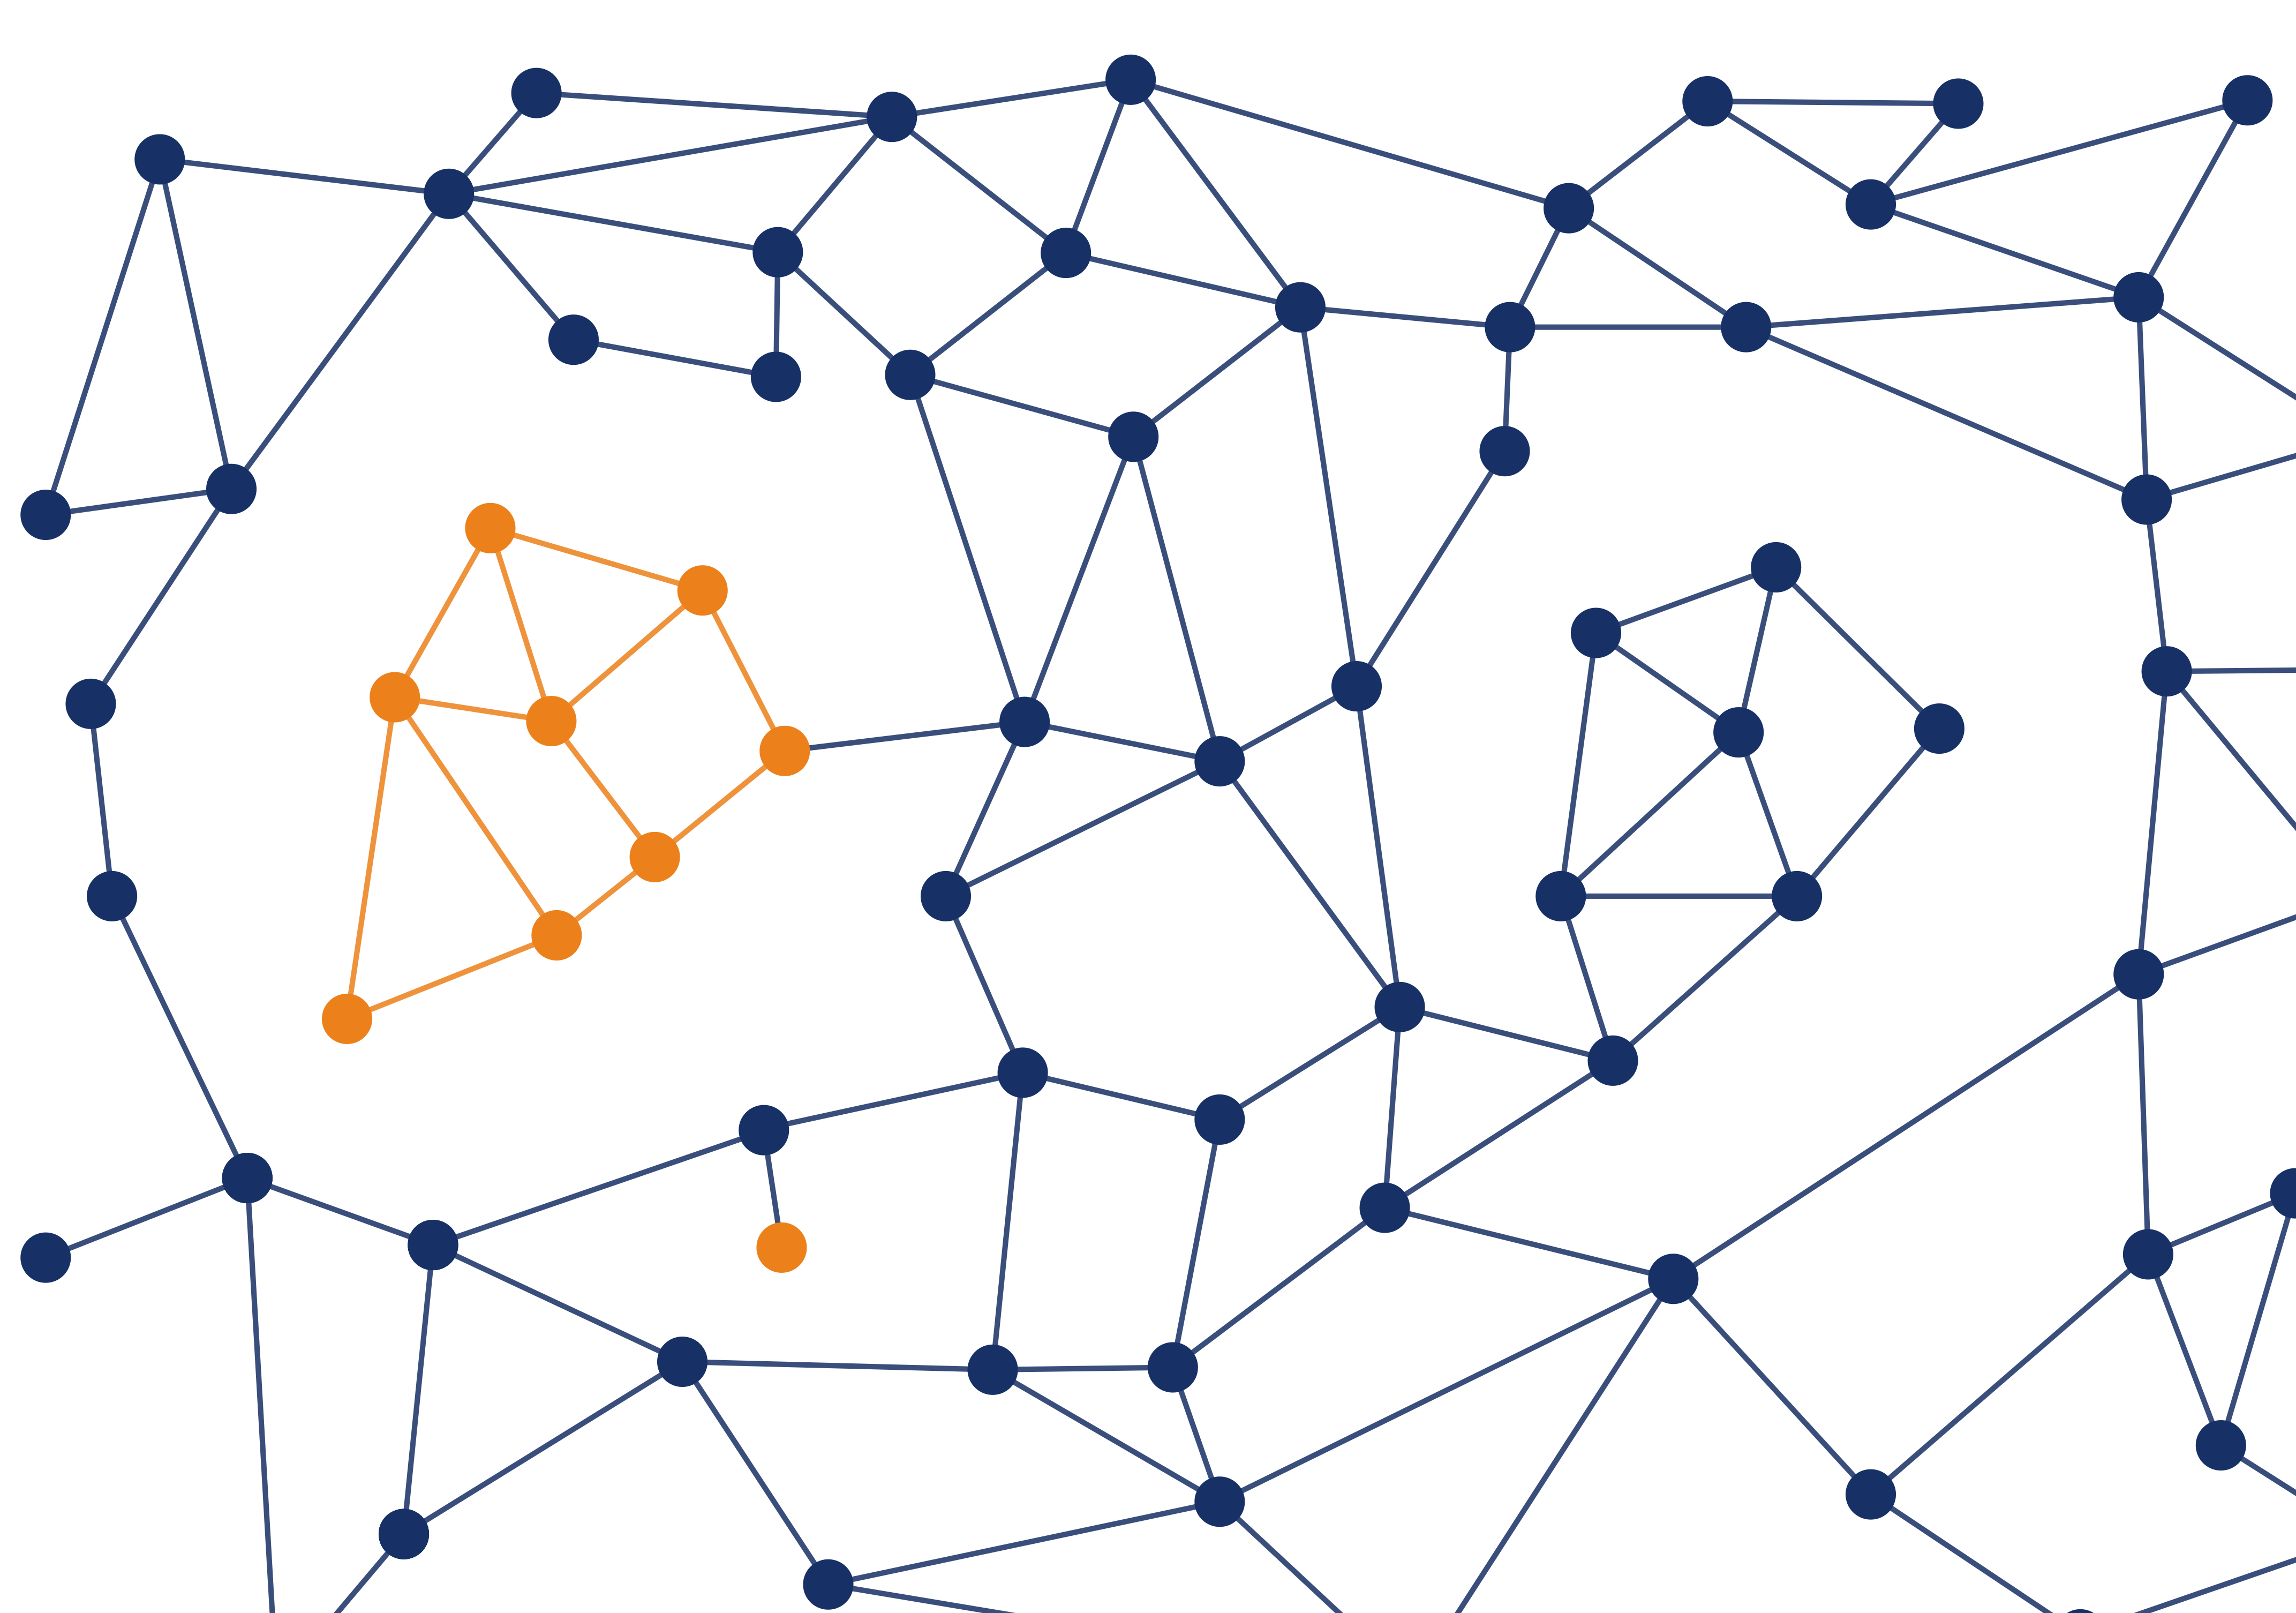
\includegraphics[width=\paperwidth]{network-with-orange}}
    \begin{frame}{Virtual Private Network}
    \end{frame}
  }
  {
    \usebackgroundtemplate{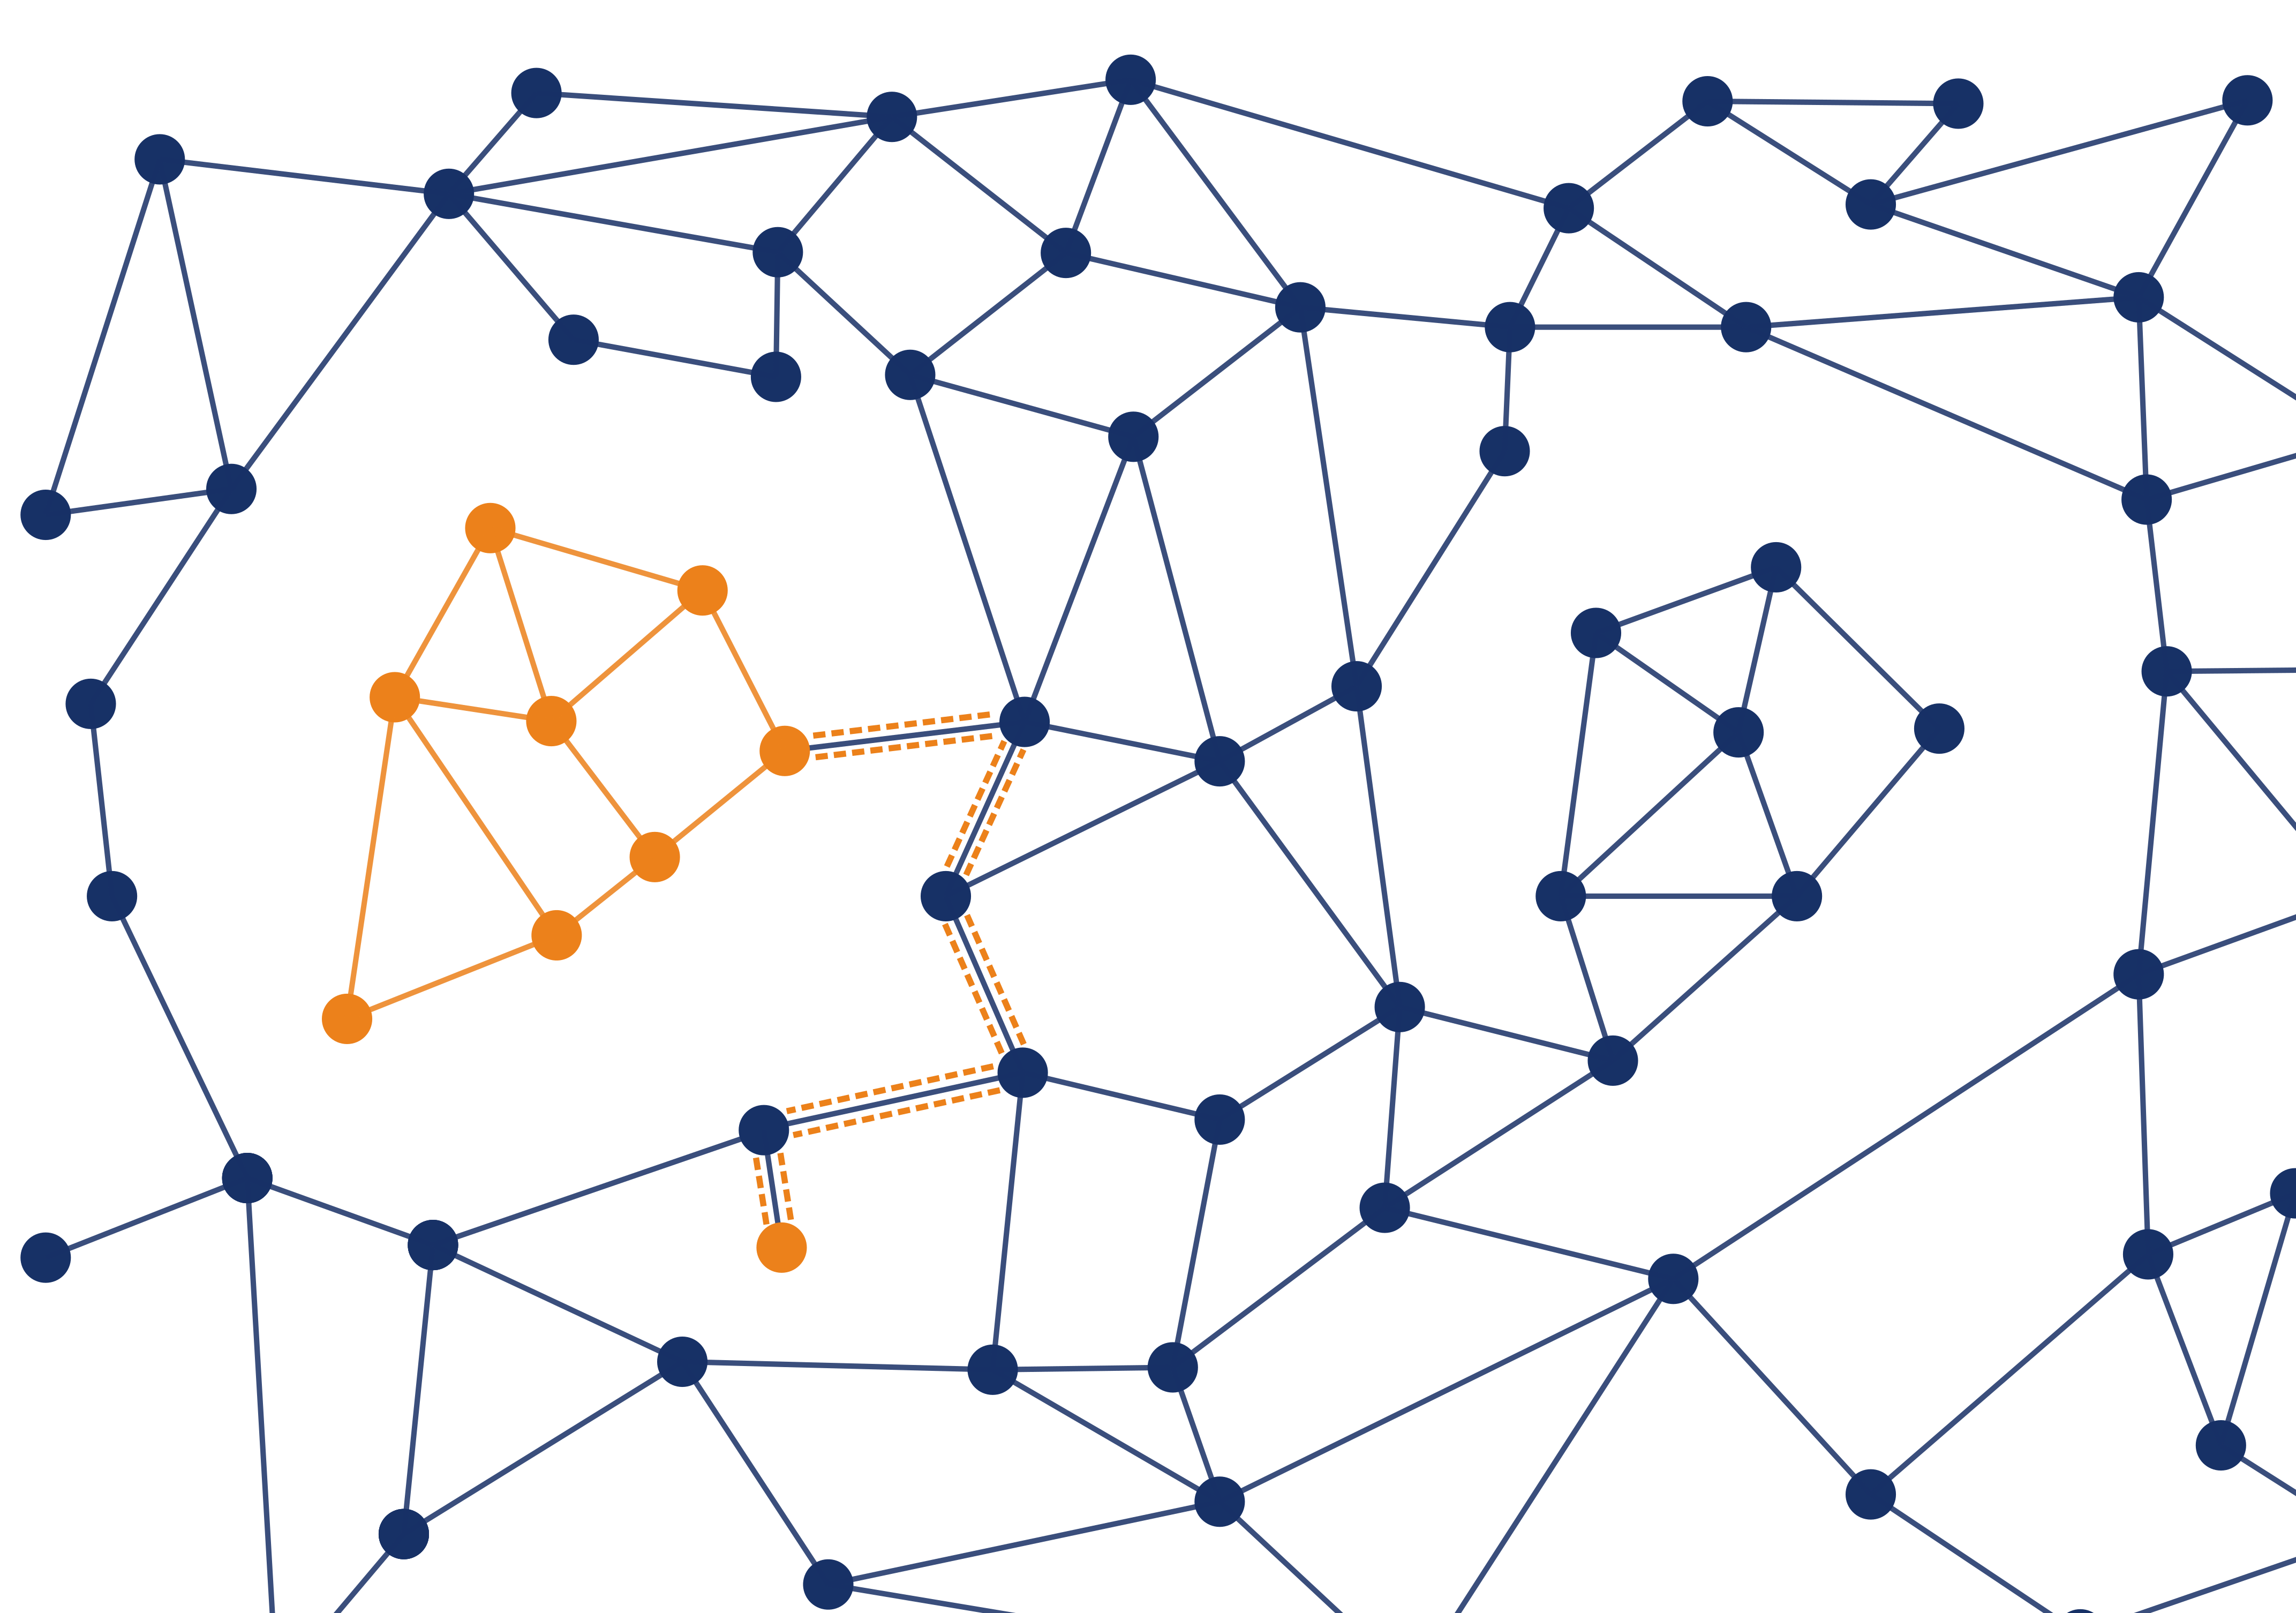
\includegraphics[width=\paperwidth]{network-with-tunnel}}
    \begin{frame}{Virtual Private Network}
    \end{frame}
  }
  {
    \usebackgroundtemplate{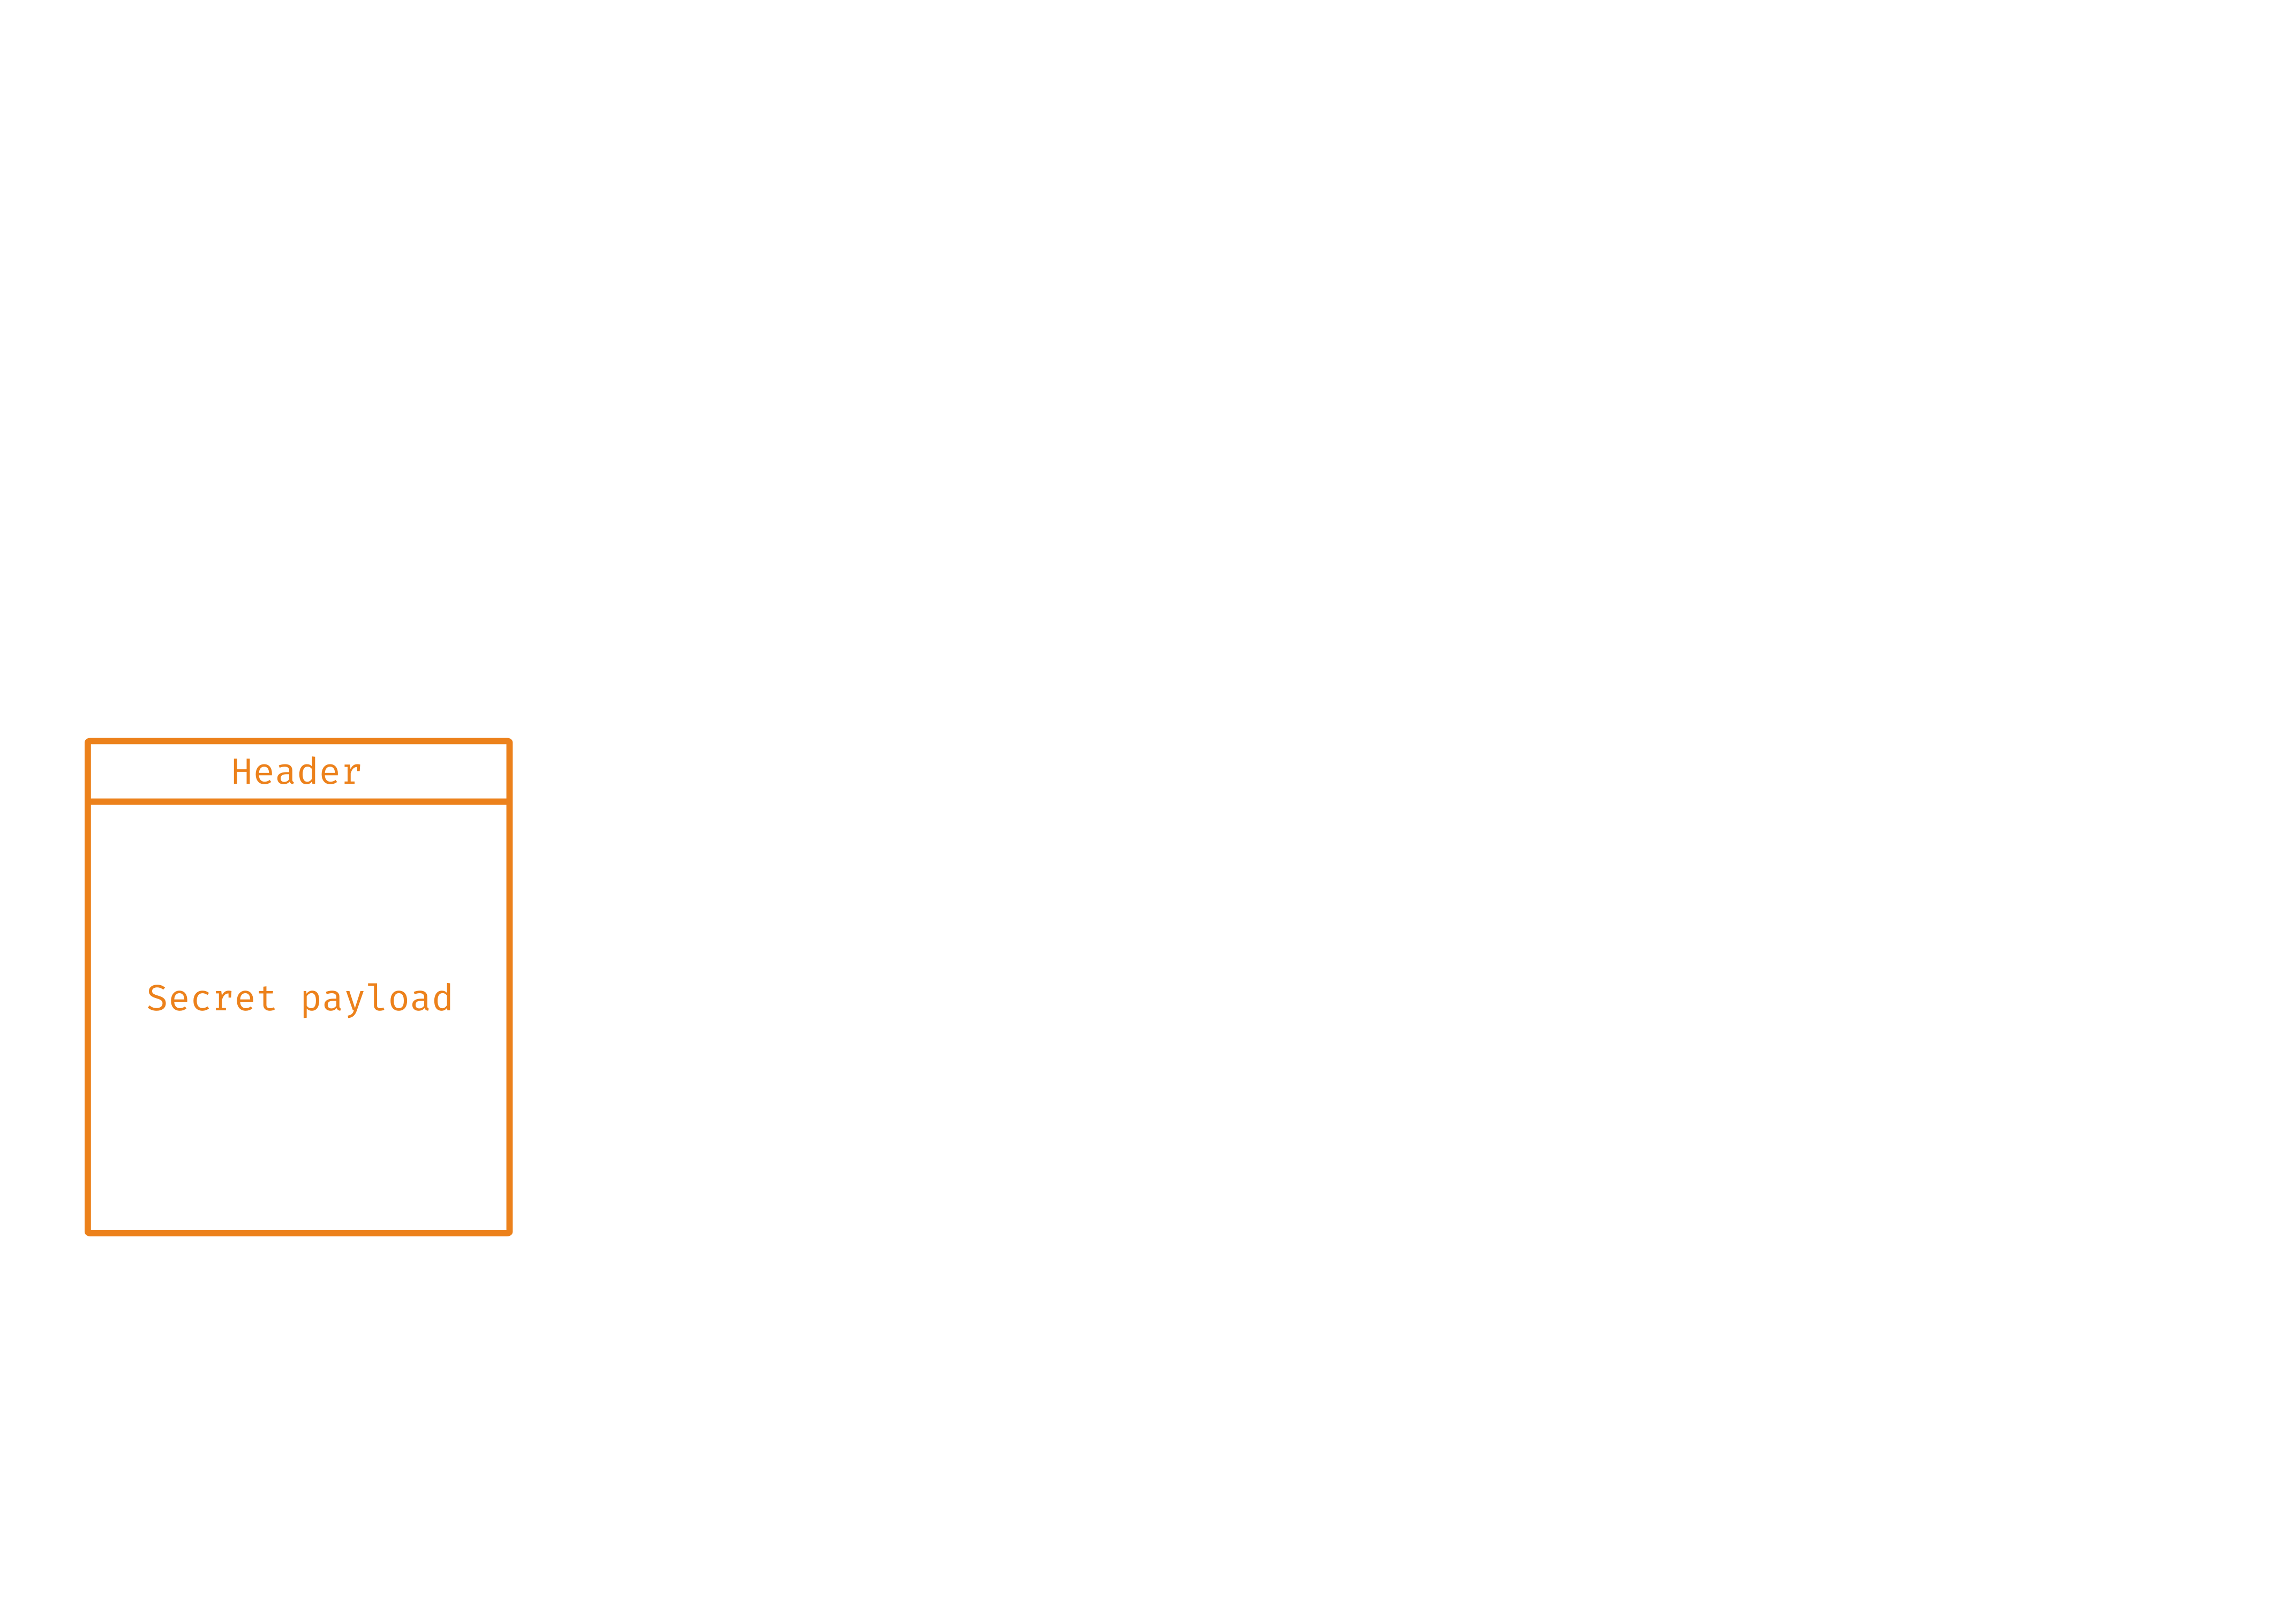
\includegraphics[width=\paperwidth]{frame-start}}
    \begin{frame}{Virtual Private Network}
    \end{frame}
  }
  {
    \usebackgroundtemplate{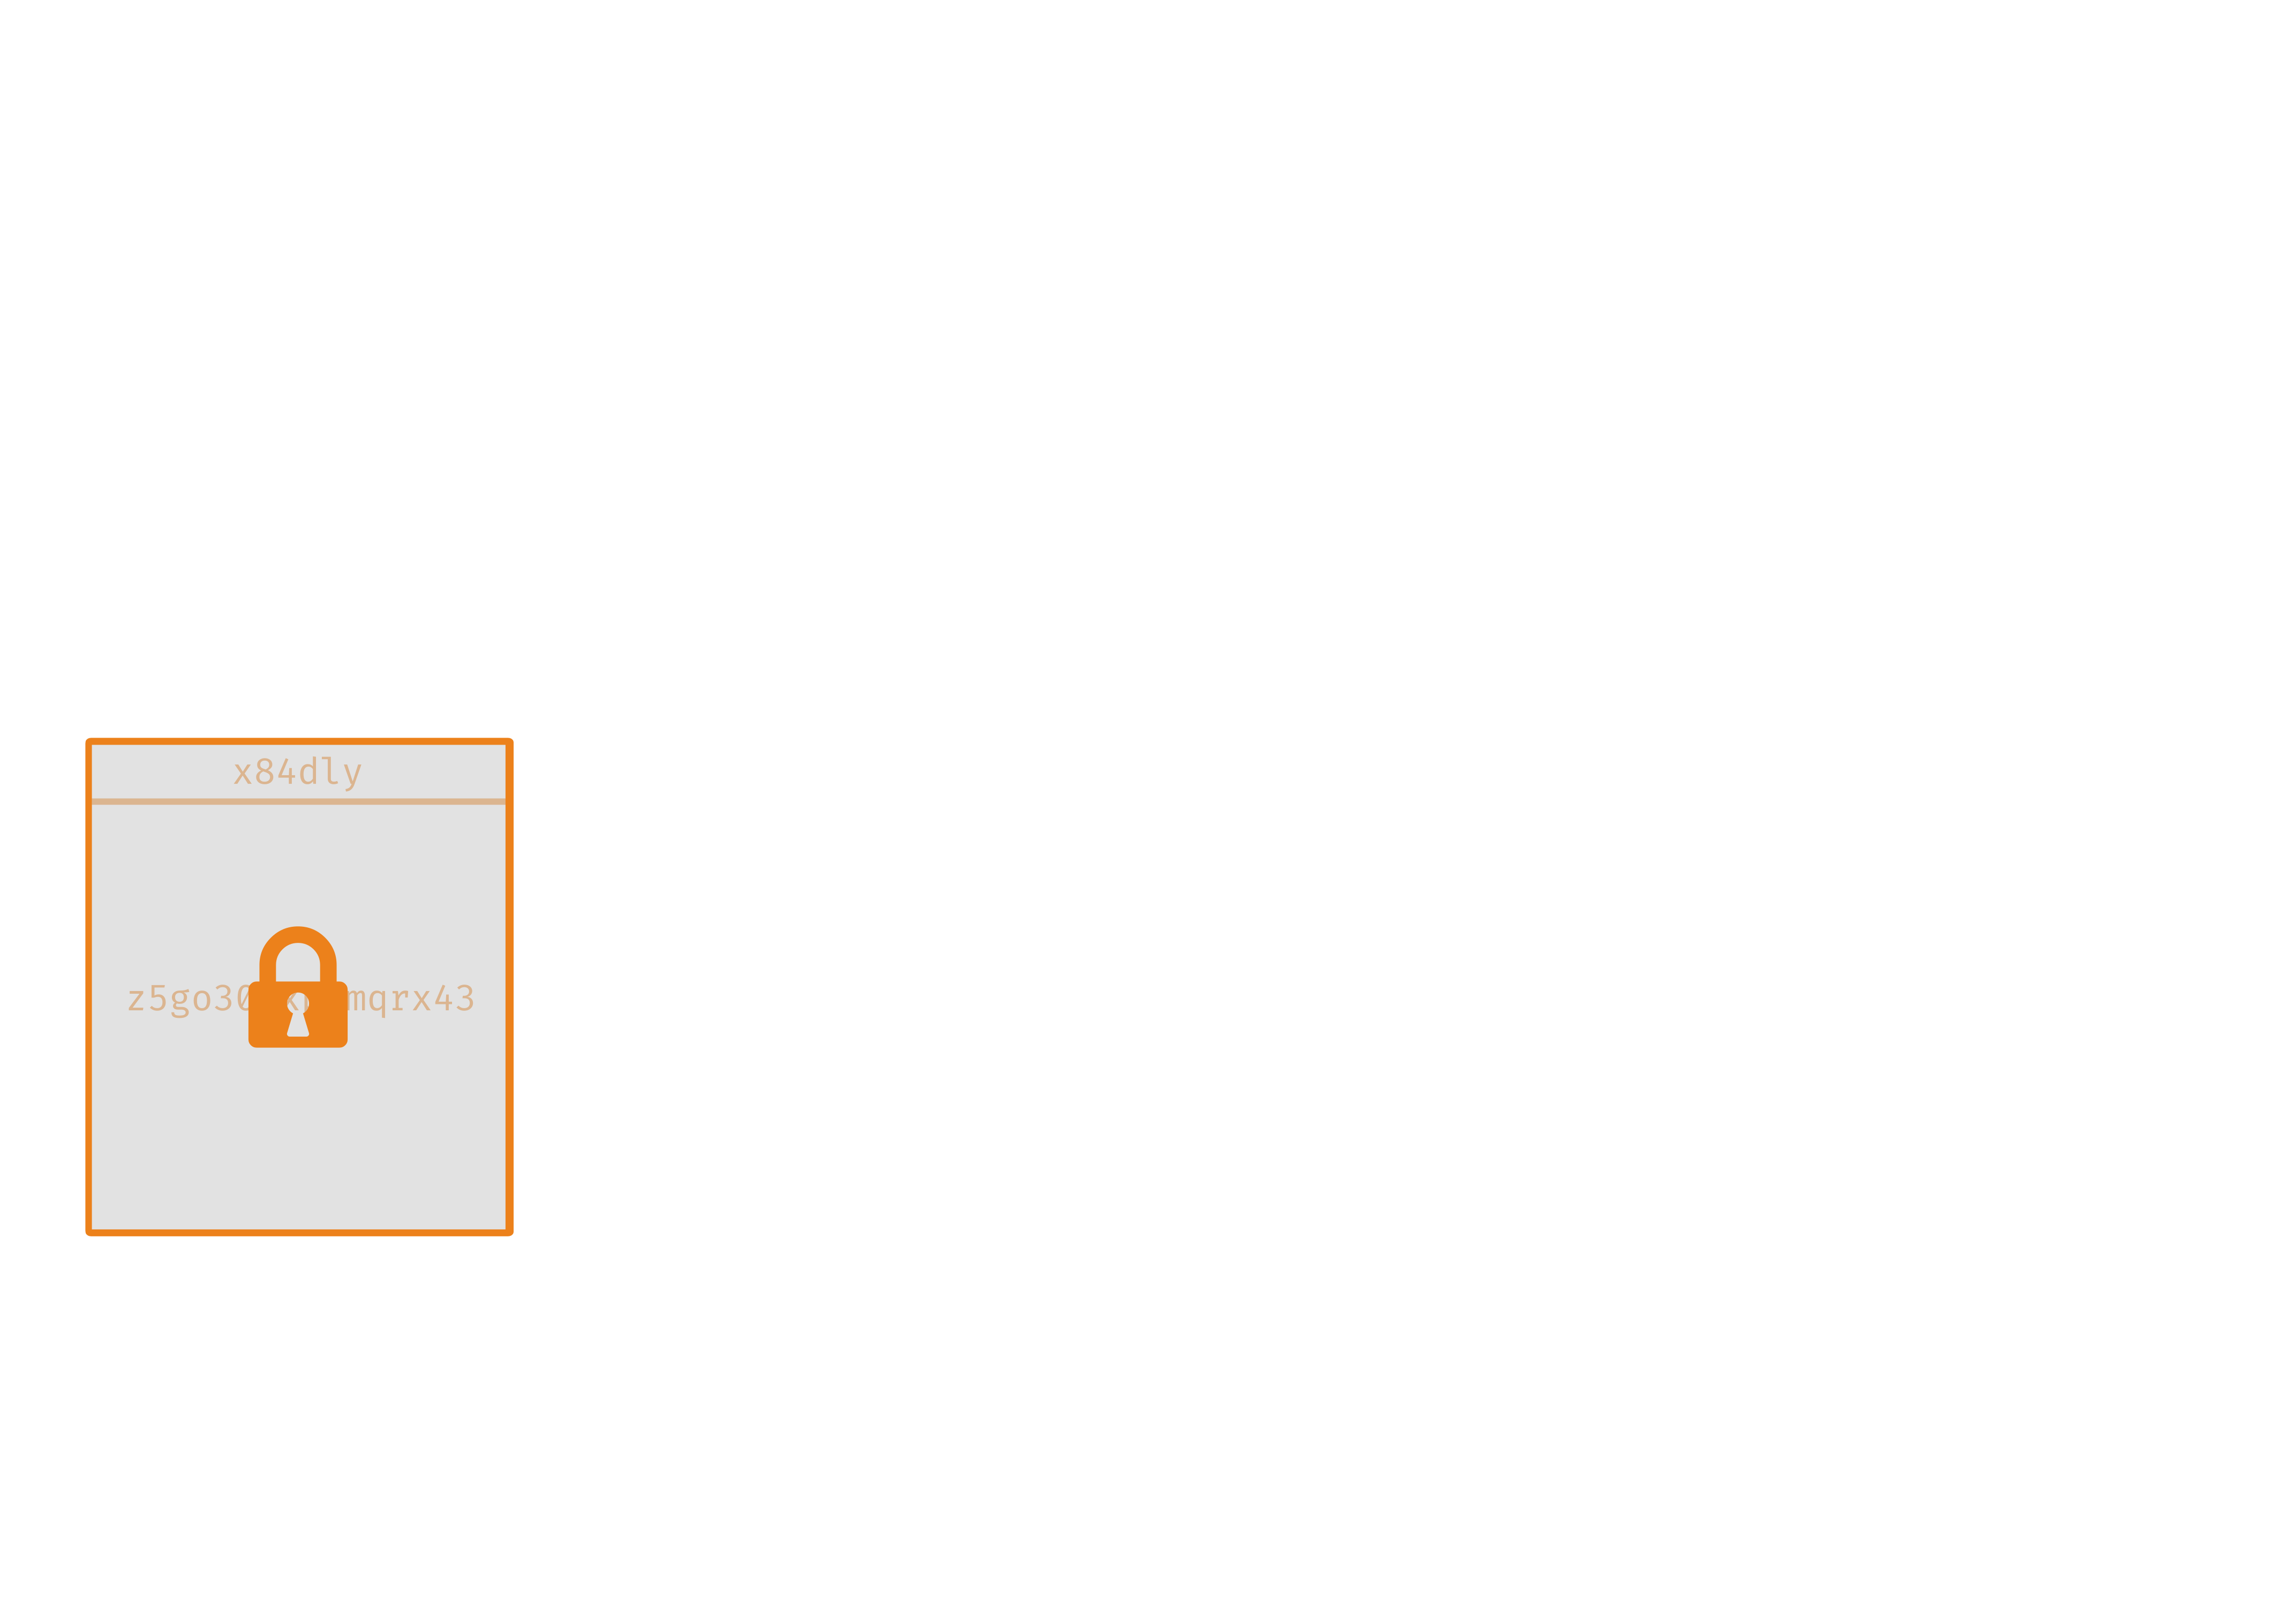
\includegraphics[width=\paperwidth]{frame-encrypted}}
    \begin{frame}{Virtual Private Network}
    \end{frame}
  }
  {
    \usebackgroundtemplate{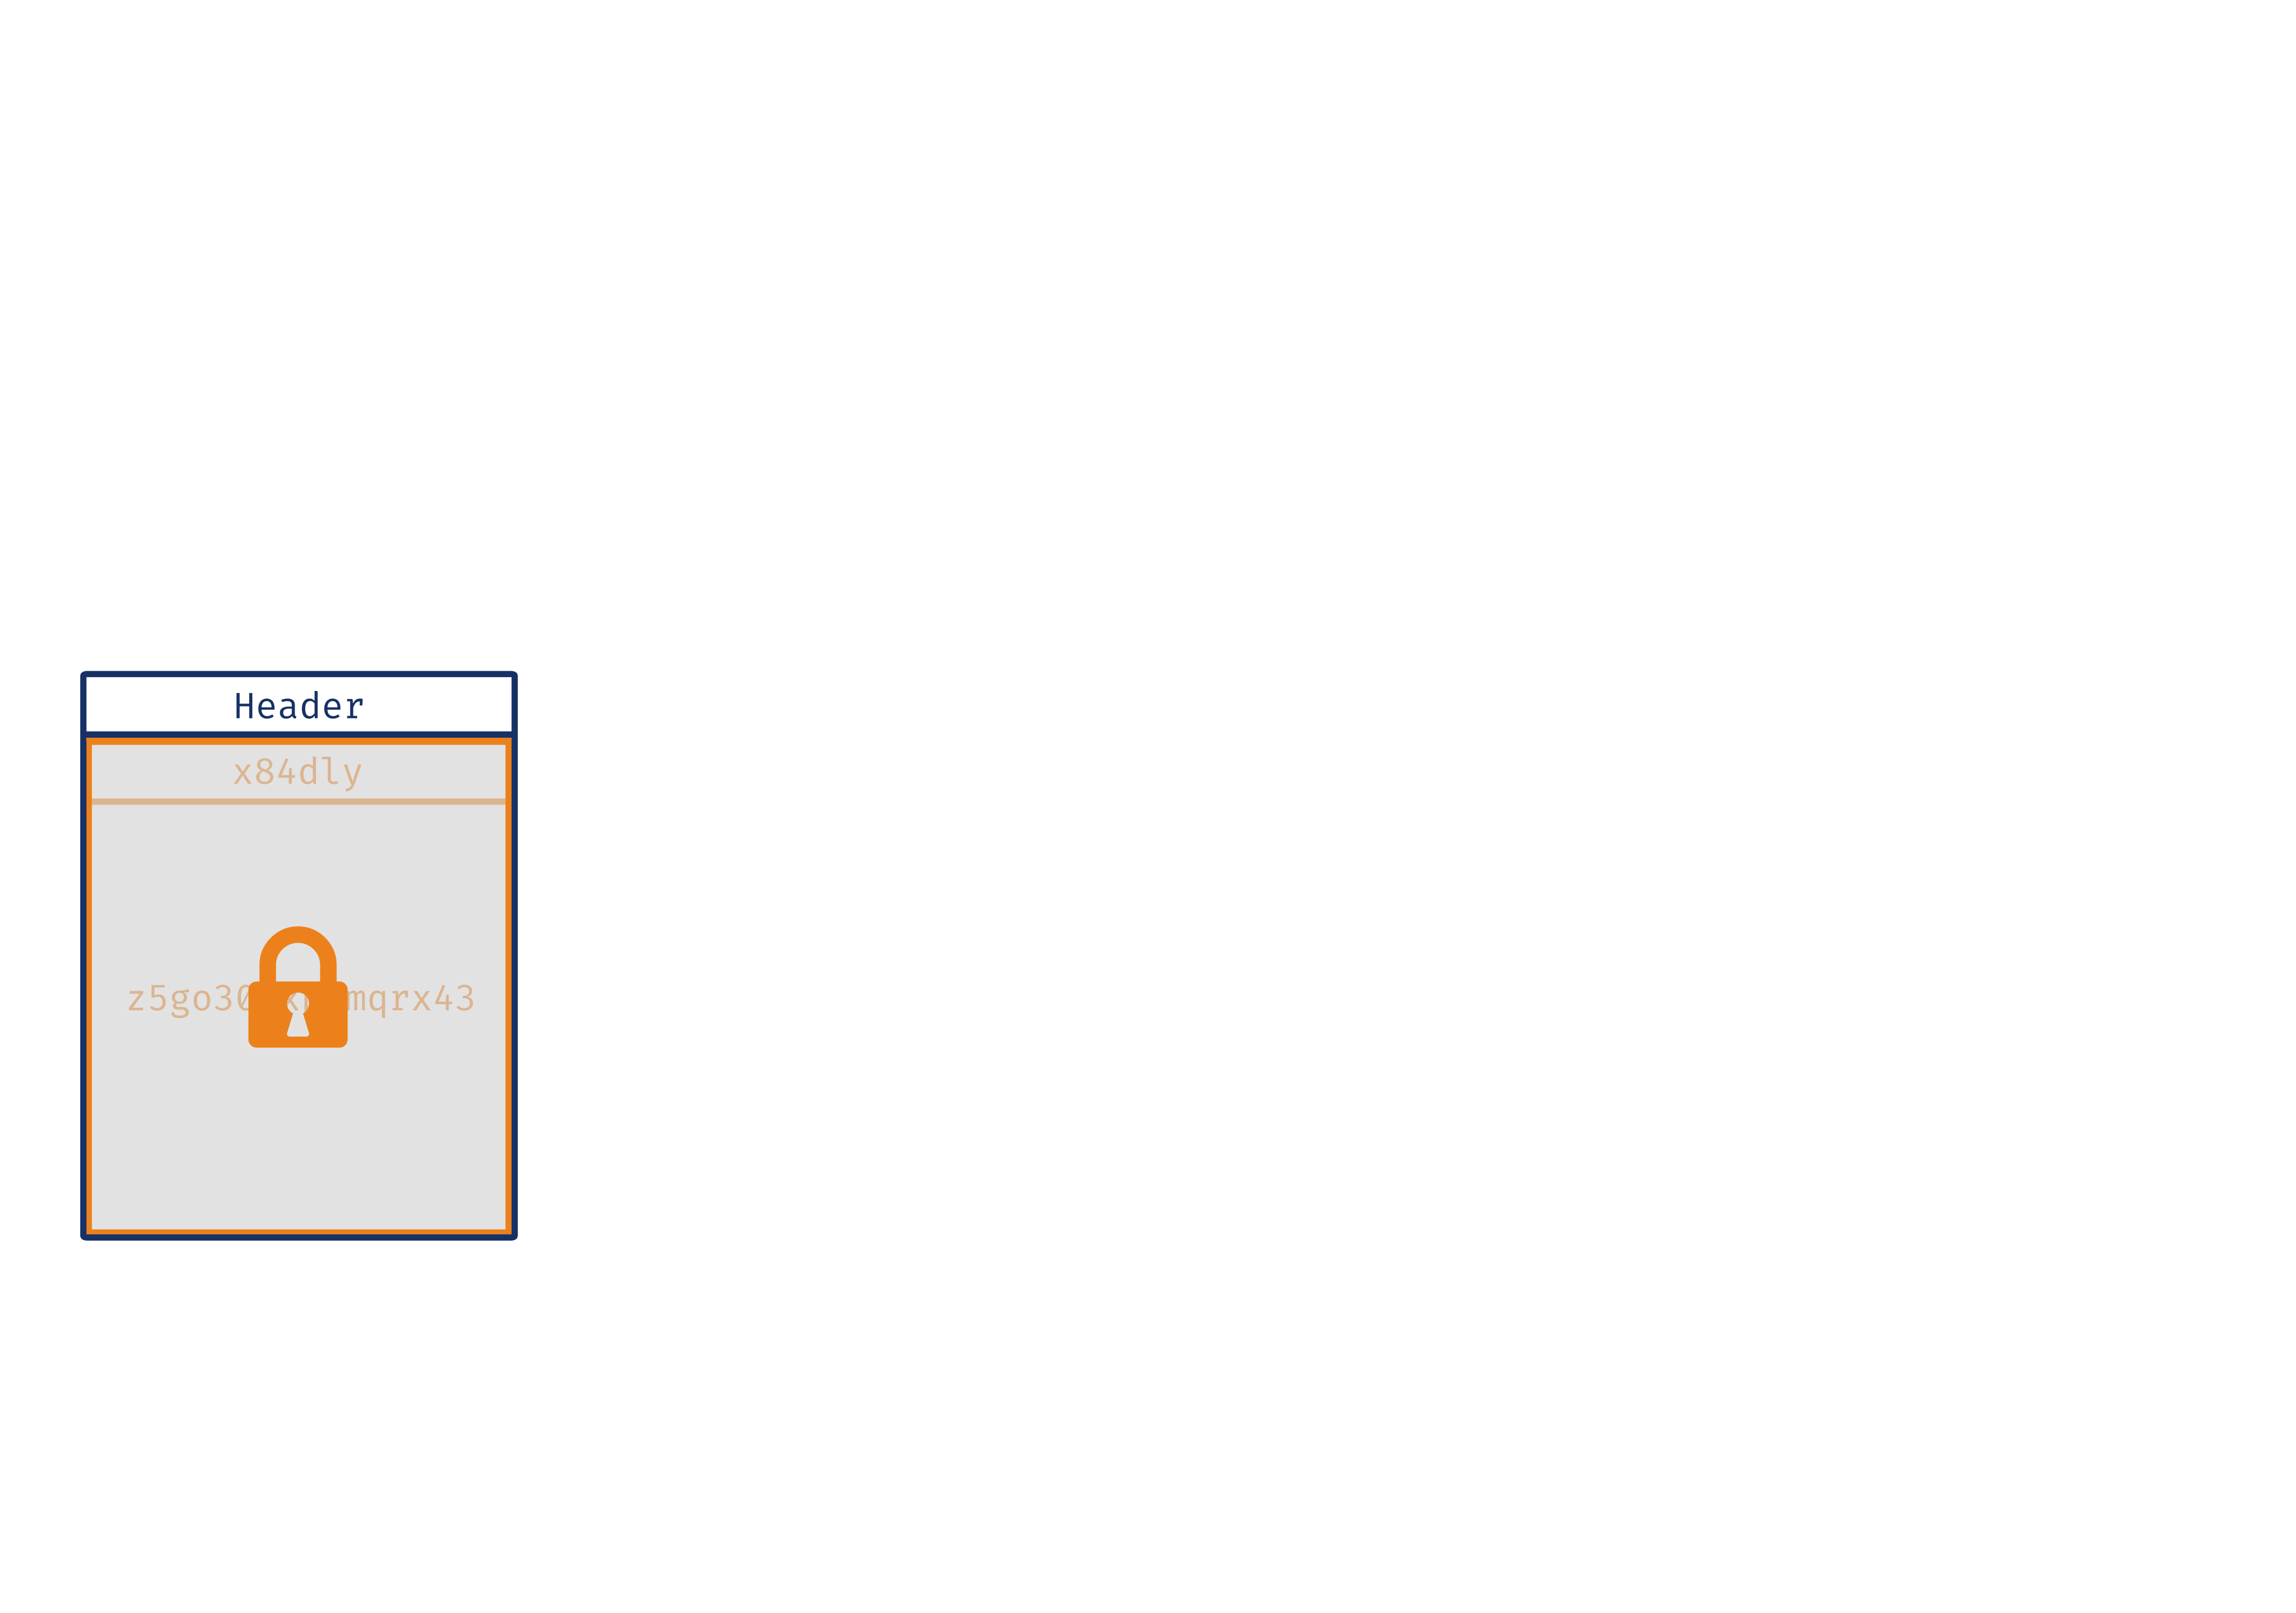
\includegraphics[width=\paperwidth]{frame-blue-header}}
    \begin{frame}{Virtual Private Network}
    \end{frame}
  }
  {
    \usebackgroundtemplate{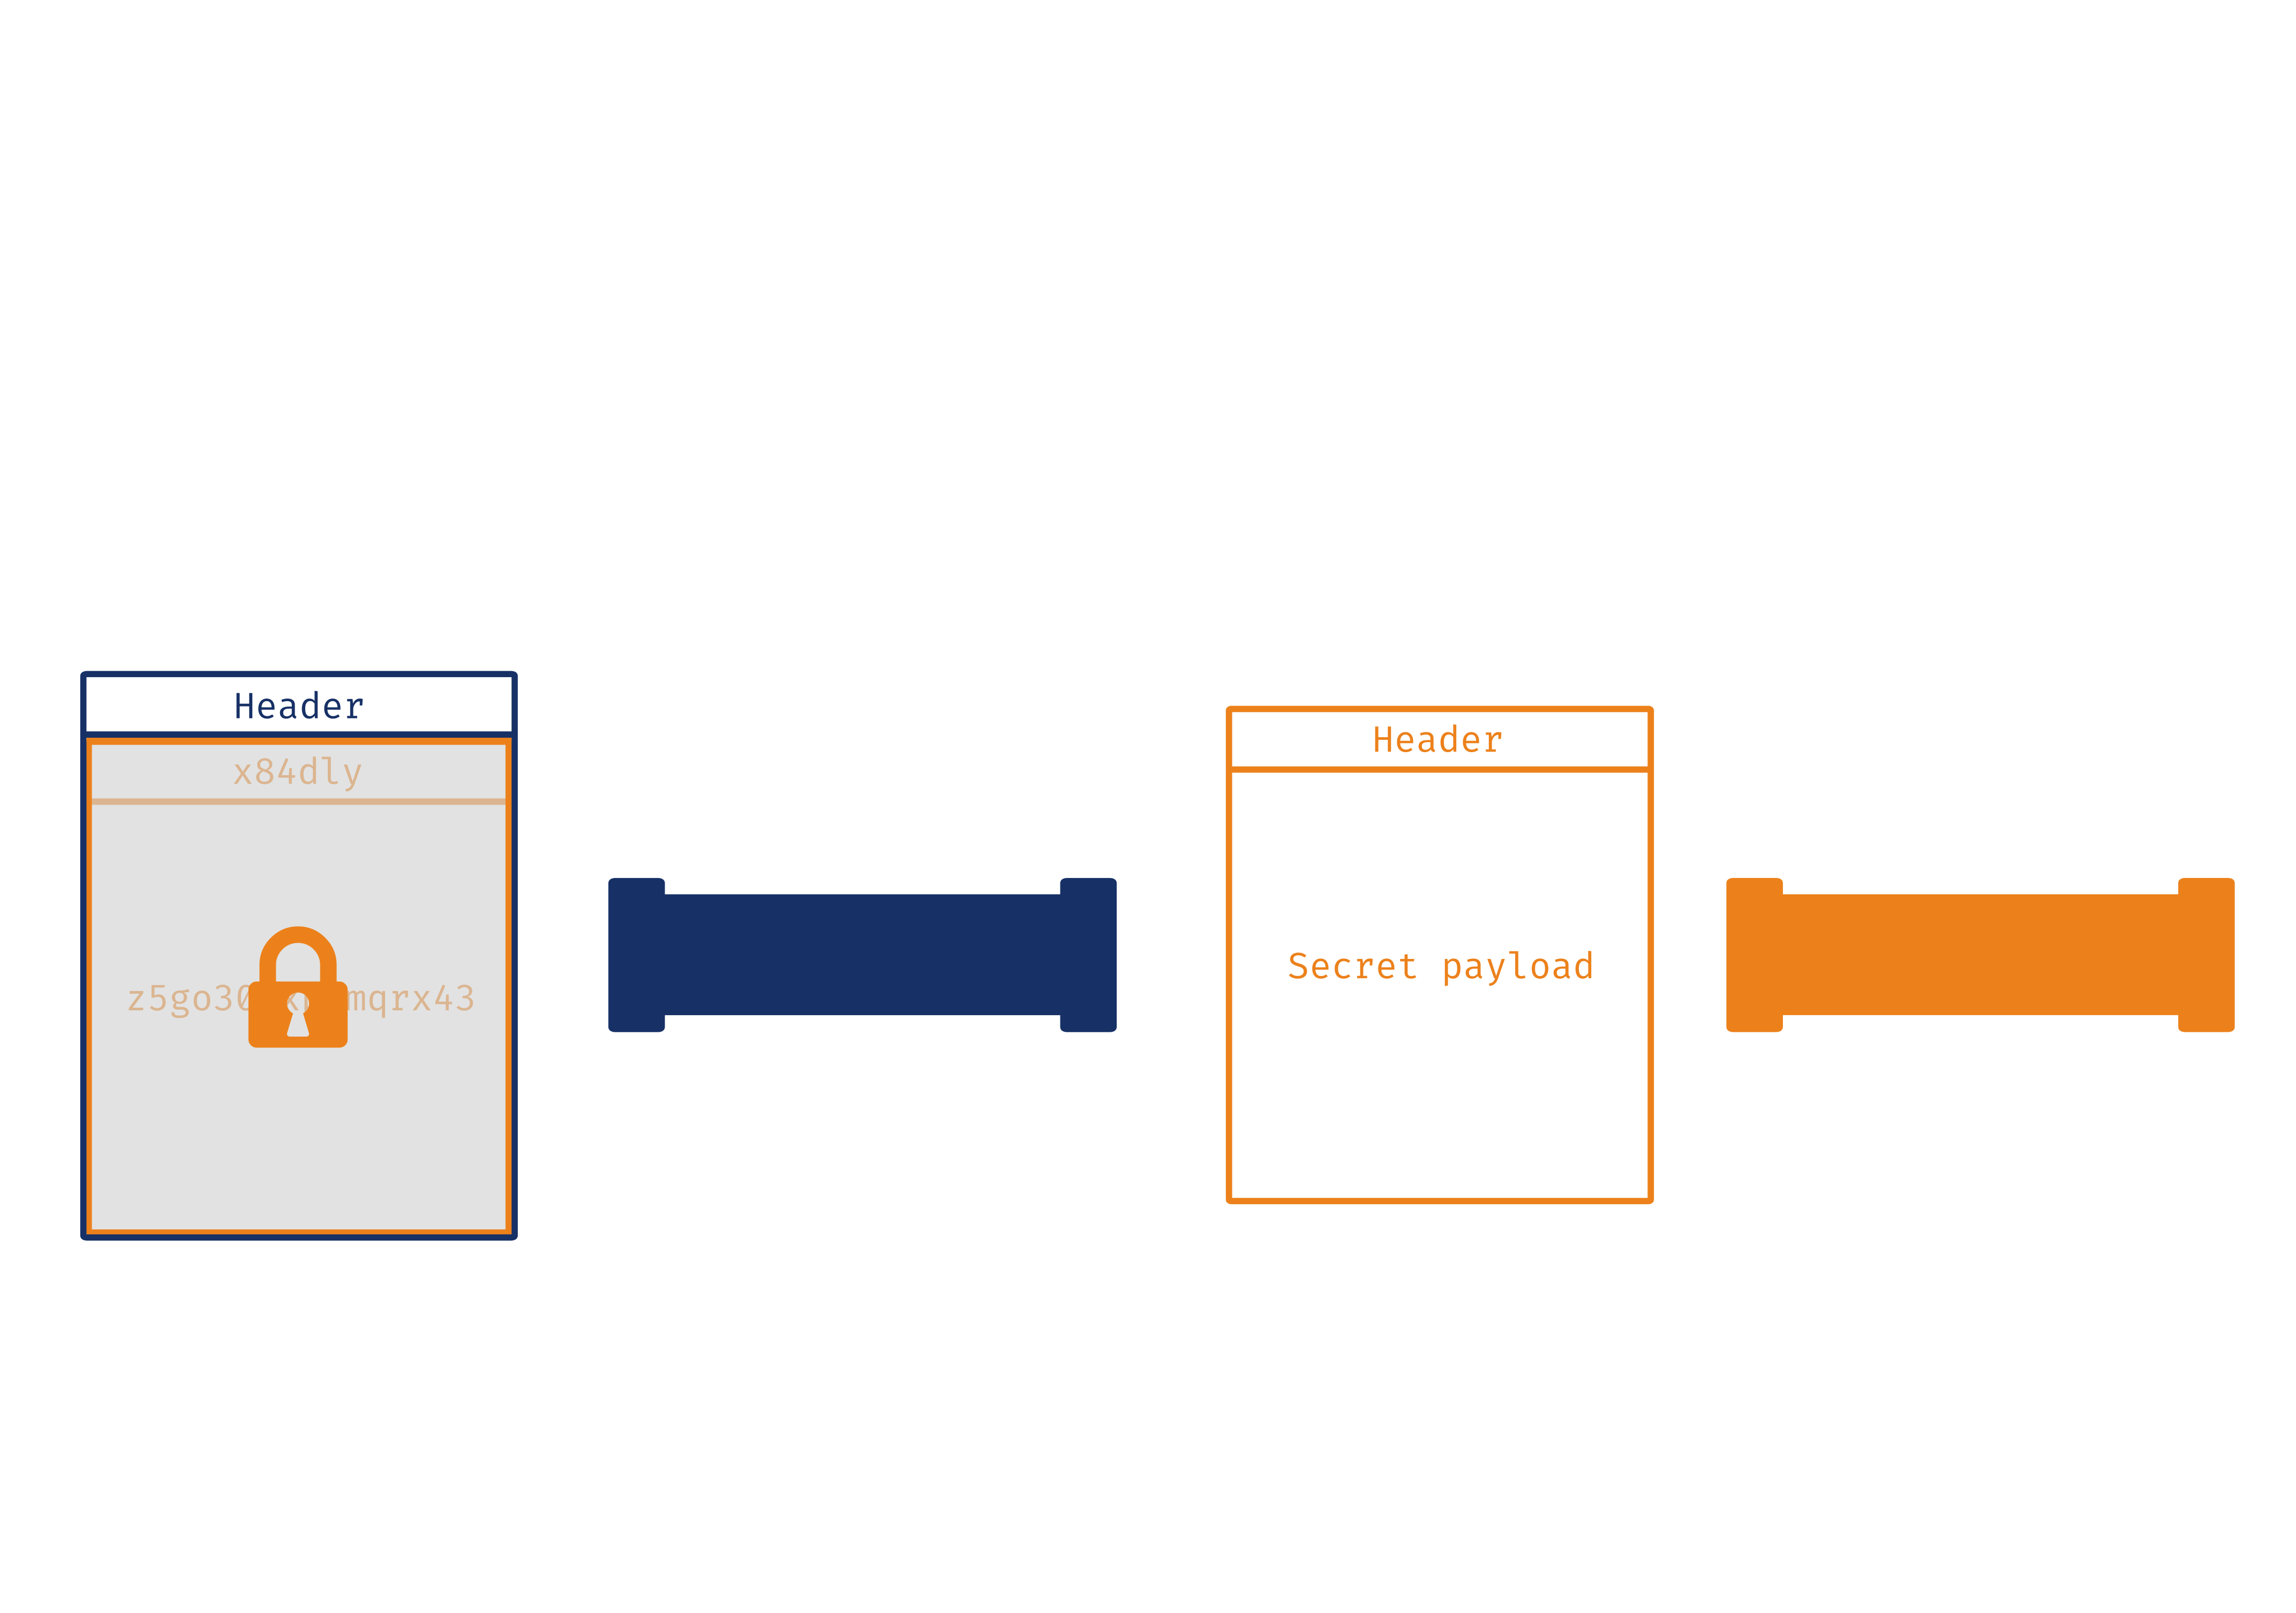
\includegraphics[width=\paperwidth]{frame-transmitted}}
    \begin{frame}{Virtual Private Network}
    \end{frame}
  }
  {
    \usebackgroundtemplate{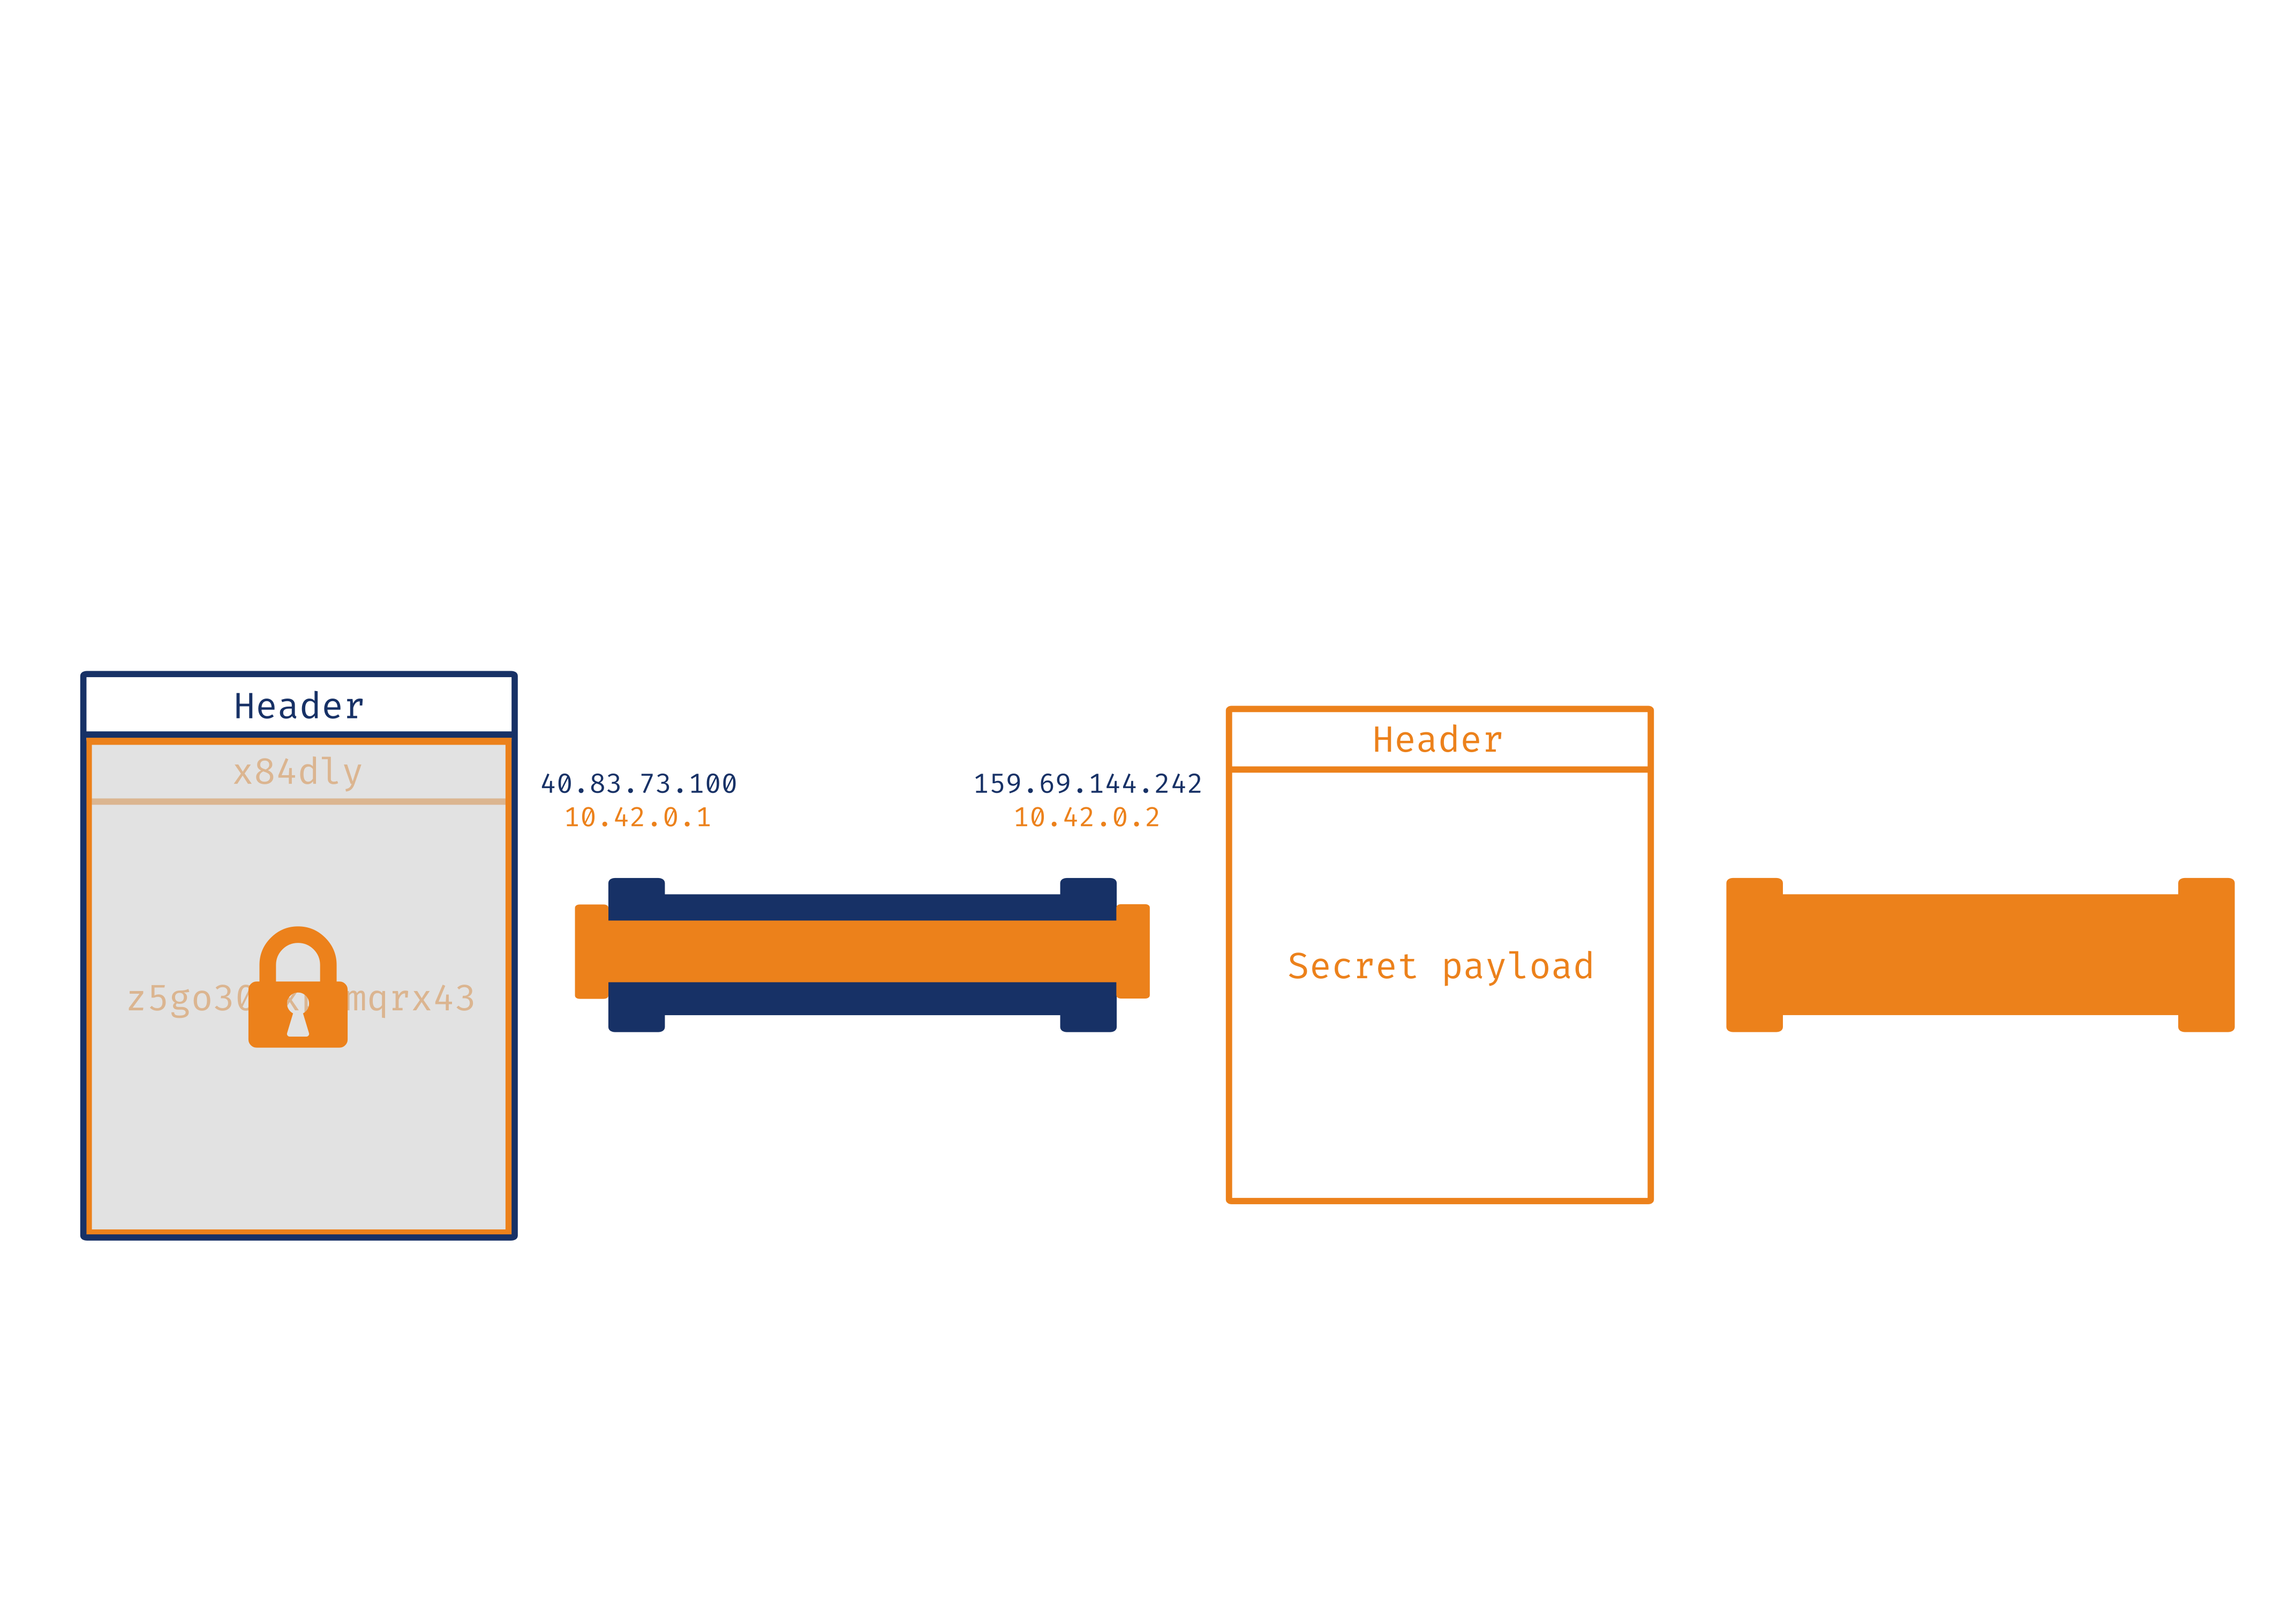
\includegraphics[width=\paperwidth]{frame-tunnel-ip}}
    \begin{frame}{Virtual Private Network}
    \end{frame}
  }

  \begin{frame}{Wozu?}
    \begin{itemize}[<+->]
      % Roadwarrior Setup
      \item Einzelne Rechner in ein Netz holen ohne physisch angebunden zu sein
      \item Firmenzentralen verbinden (site to site)
      \item Privatsphäre in offenen Netzwerken
      \item \grqq{Anderes Internet} z.B. zur Umgehung von Geoblocking
    \end{itemize}
  \end{frame}


  \section{Wie macht man das?}

  \begin{frame}{Zum Beispiel mit Wireguard}
    
\includegraphics[width=\textwidth]{wireguard}
  \end{frame}

  \begin{frame}{Was ist Wireguard?}
    \begin{itemize}
      \item Neue, simples Layer 3 VPN mit moderner Verschlüsselung
      \item Basierend auf UDP
      \item Läuft im Linux Kernel und ist sehr performant
      \item Einfach zu nutzen
      \item Stealthy 
    \end{itemize}
  \end{frame}
  \begin{frame}{Authentifizierung}
    \begin{itemize}
      \item Sehr ähnlich zu SSH
      \item Jeder Teilnehmer generiert sich einen Private- und Public-Key
      \item Der Public Key wird mit allen geteilt
    \end{itemize}
  \end{frame}

  \begin{frame}[standout]
    Demo
  \end{frame}

  \begin{frame}{Kryptokey Routing}
    \begin{itemize}[<+->]
      \item Jeder Teilnehmer hat eine Liste von Peers mit deren Public-Key und erlaubten \alert{Tunnel} IP-Adressen
      \item Wenn ein Paket verschickt werden soll sucht Wireguard nach dem Peer mit der IP und verschlüsselt mit dessen Public-Key
      \item Wenn Wireguard ein Paket erhält wird überprüft ob es von einer gültigen Tunnel IP und Public-Key Kombination kommt. Nut dann wird es angenommen
      \item Das garantiert, dass jedes Paket für eine bestimmte Tunnel IP das von Wireguard kommt, sicher nur von dem richtigen Peer kommen kann
    \end{itemize}
  \end{frame}
  \begin{frame}{Kryptokey Routing}
    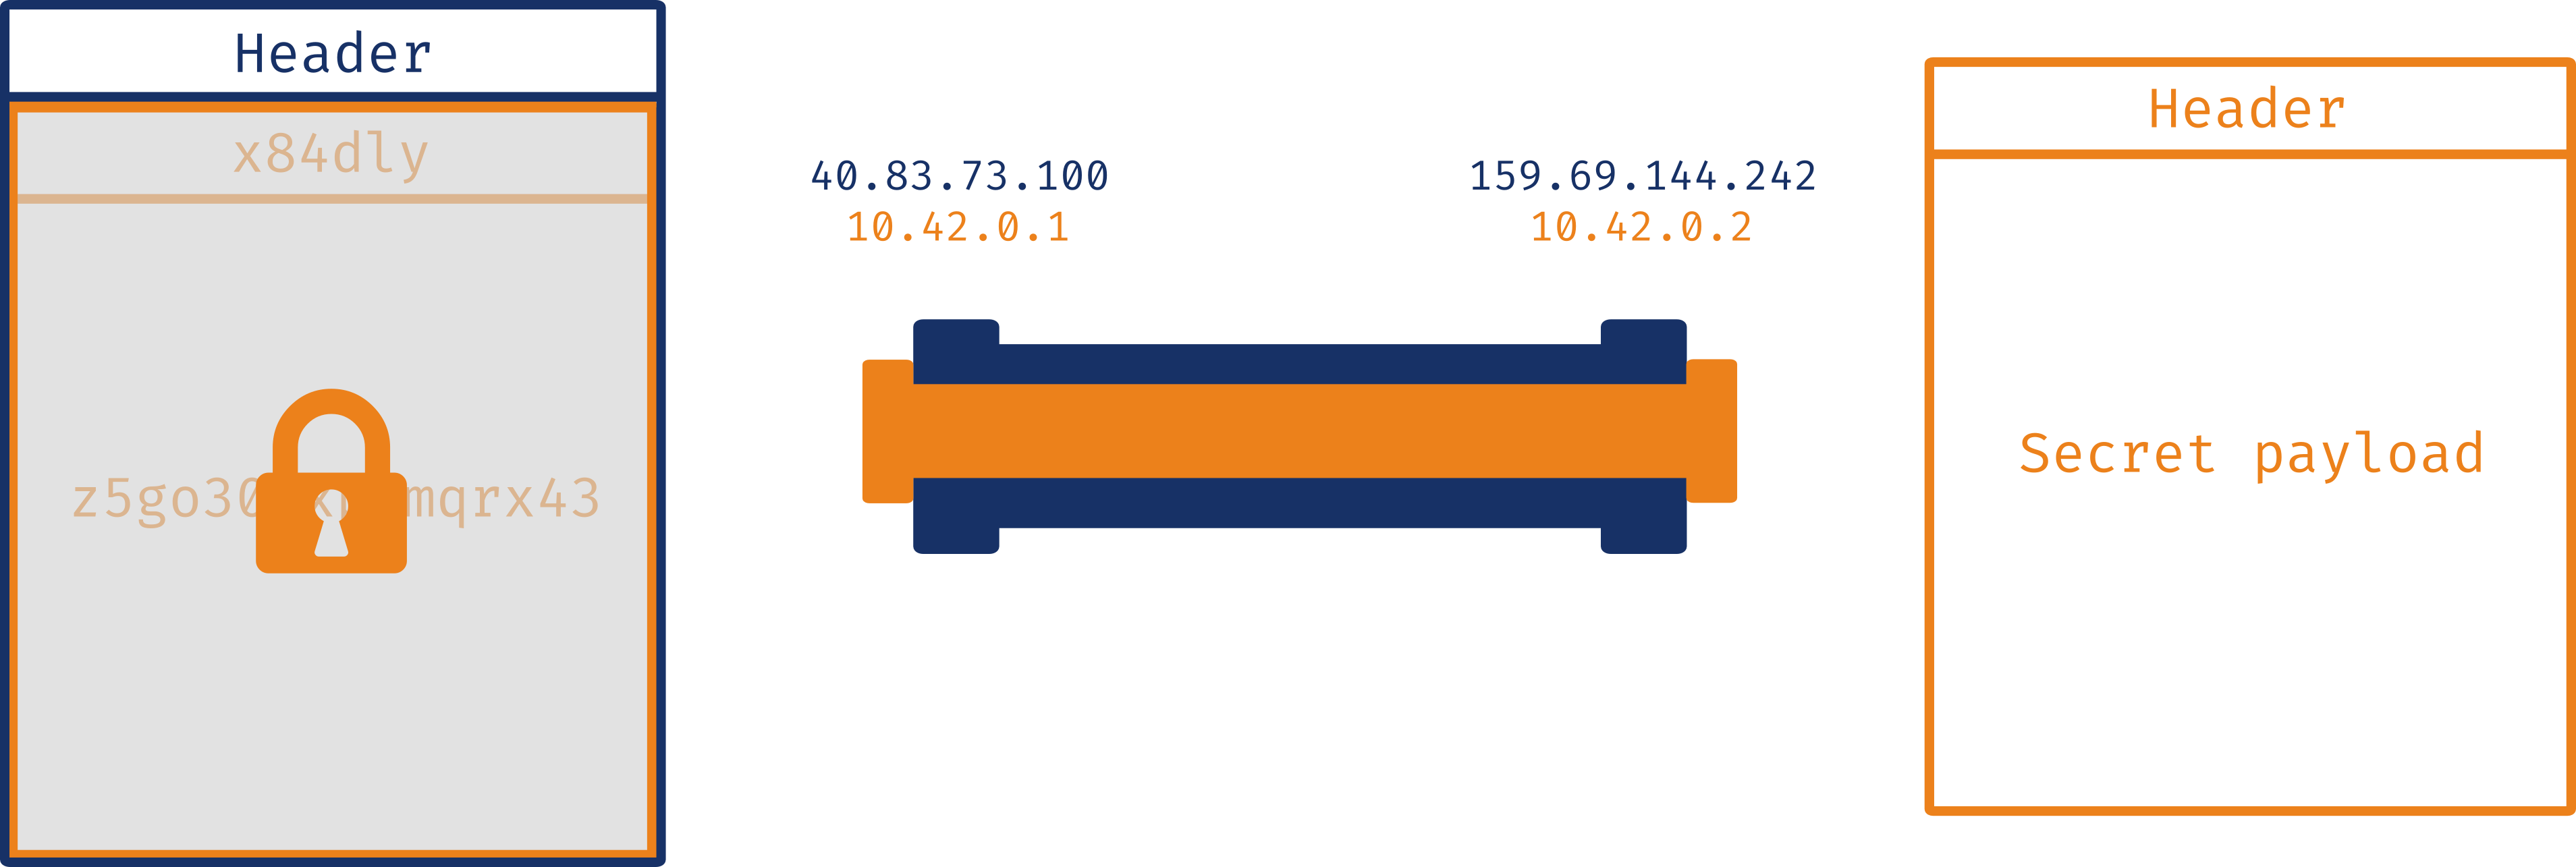
\includegraphics[width=\textwidth]{kryptokey-pre}
  \end{frame}
  \begin{frame}{Kryptokey Routing}
    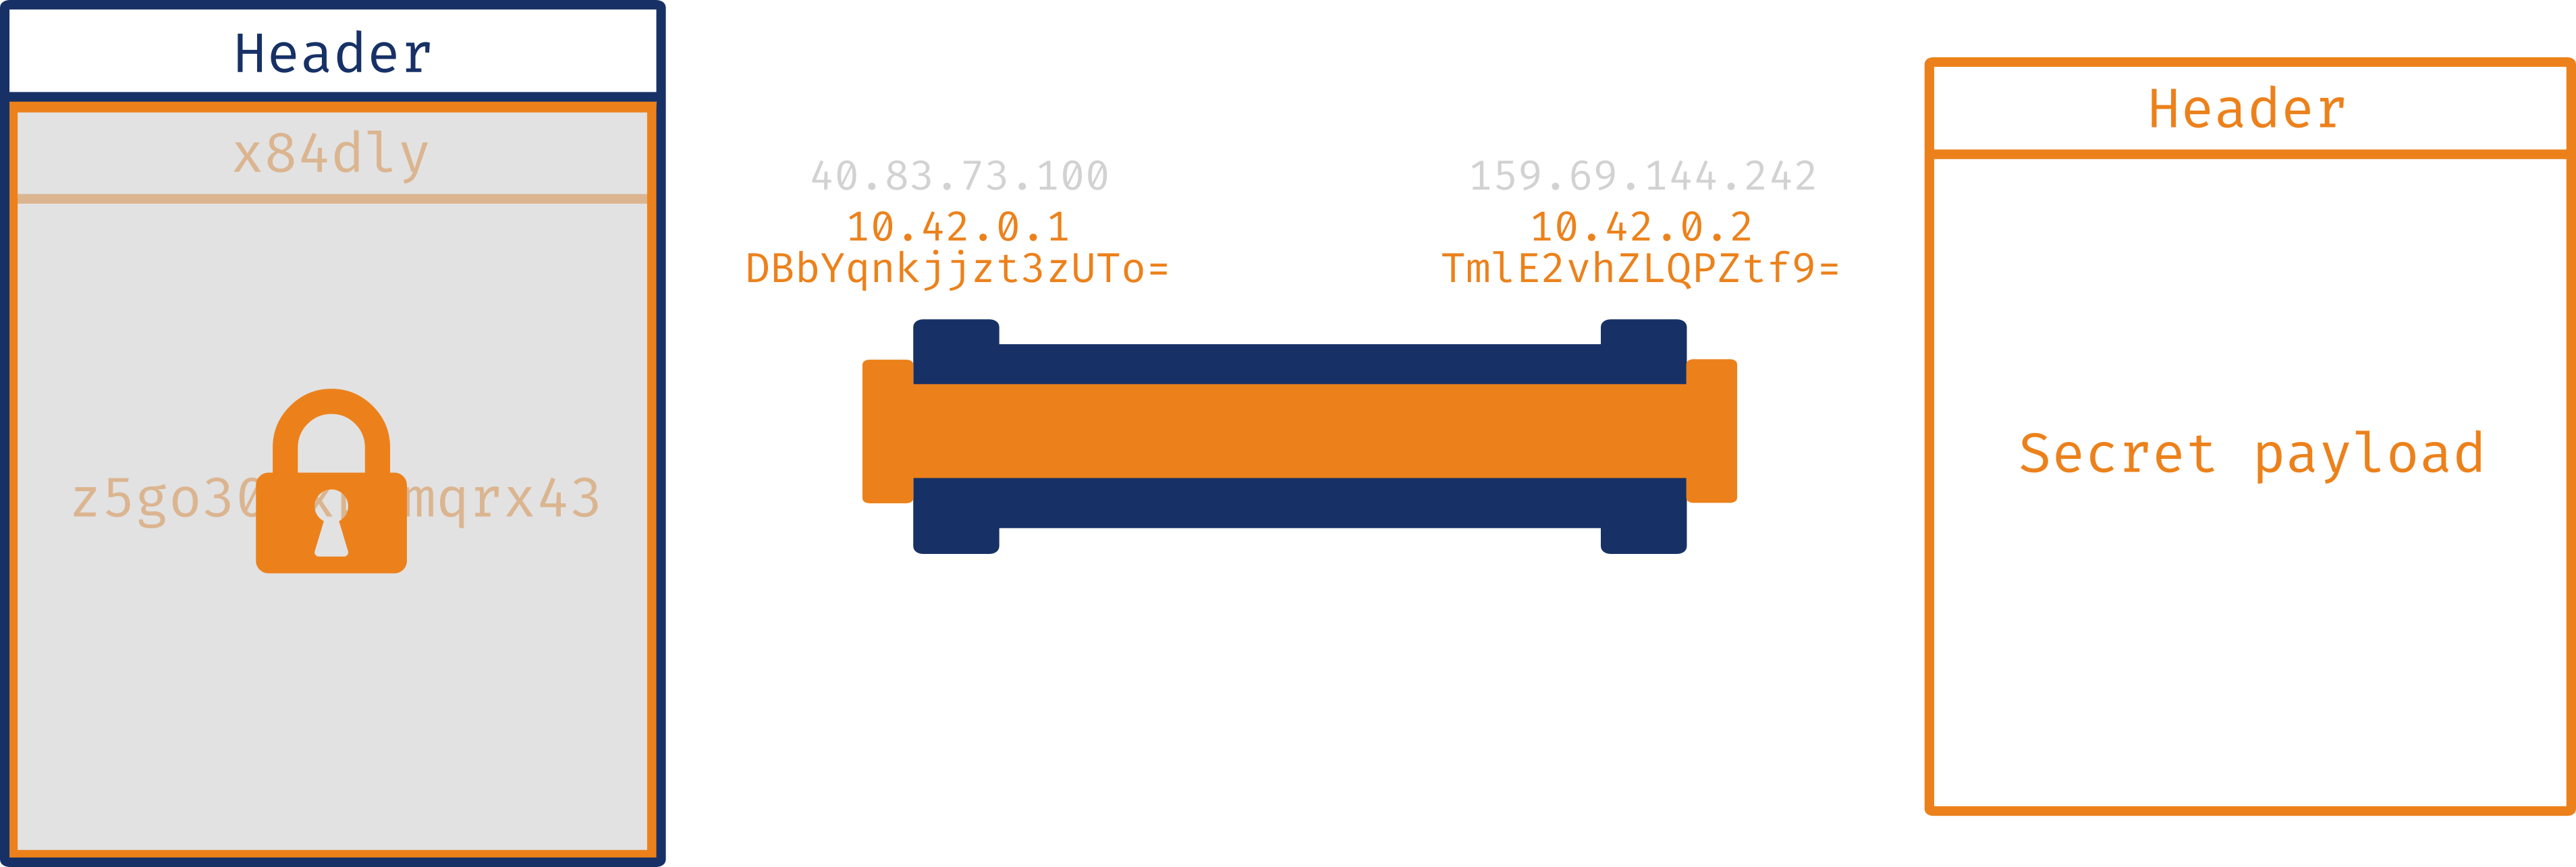
\includegraphics[width=\textwidth]{kryptokey}
  \end{frame}

  \begin{frame}[standout]
    Mehr Demo
  \end{frame}

  \begin{frame}[standout]
    
\includegraphics[width=0.7\linewidth]{cio-logo} \\
    Vielen Dank! Fragen? \\
    @AnianZ \\
  \end{frame}

  \begin{frame}{Wichtige Quellen und Tutorials}
    \begin{itemize}
      \item Requests for comments Podcast über VPNs: https://requestforcomments.de/archives/682
      \item Wireguard hompage: https://www.wireguard.com/
      \item Wireguard vom Author vorgestellt: https://youtu.be/CejbCQ5wS7Q
      \item Wireguard setup tutorial: https://www.stavros.io/posts/how-to-configure-wireguard/
      \item IP Forwarding in Linux: http://www.ducea.com/2006/08/01/how-to-enable-ip-forwarding-in-linux/
      \item Un-Official Wireguard docs: https://github.com/pirate/wireguard-docs#Dynamic-IP-Allocation
      \item TechSnap Podcast Folge über Wireguard: https://techsnap.systems/403
    \end{itemize}
  \end{frame}
  % - Einzelne Rechner in ein Netz holen ohne physisch angebundnen zu sein. z.B. Zugang zum Uni Netz -> Privates Netzwerk
  %   - Roadwarrior Setup
  % - Firmenzentralen (netze) verbinden -> site to site
  % - Privatsphäre  in offenen Netzwerken, Port manchmal port blocking umgehen 
  % - Anderes Internet, umgehung von Geoblocking 
  
  % https://requestforcomments.de/archives/682
  % - Man hat immer 2 IP Adressen: Außererhalb des Tunnels und innerhalb
  % - Vorsicht: Tunnel endpunkte nicht über den Tunnel routen
  % - MTUs ethernet 1500 => drinnen kleiner "ping geht, browser bleibt stecken" siehe Deutsche Bahn
  %   - DSL 1492

  % - VPN ist nicht immer verschlüselt, notwendigerweise
  % - Schlüsselmaterial muss ausgetauscht werden
  %   - Pre-Shared keys
  %   - Zertifikate

  % - Außen: Meist UDP
  % - Dann VPN protokoll
  % - dann innerer Prozess

  % - Mobility: Äußere IP kann wechslen (Roaming)

  % - Userspace vs Kernel Space implementierungen
  
  % - Punkt zu Punkt oder Punkt zu mehrpunkt? Wireguard ist punkt zu mulipunkt
  %   - Kryptokey-routing anstatt IP addressen
  
  % Was wird innerhalb getunnelt? Gibt alles von Layer 2 zu Layer 4
  %   - Wireguard macht nur Layer 3, kein virtuelles Ethernet

  % Dynamische routing protokolle sind schwer mit Wireguard


\end{document}
